\documentclass[a4paper, 10.5pt, oneside, openany, uplatex]{jsarticle}

\author{山内 仁喬}
% 余白の設定.
% 参考文献:Latex2e 美文書作成入門, 14.3ページレイアウトの変更

% 行長の変更
\setlength{\textwidth}{40zw}           %全角40文字分

% 行間を制御するコマンド
\renewcommand{\baselinestretch}{0.9}

% 左マージンを変更
\setlength{\oddsidemargin}{25truemm}   % 左余白
\addtolength{\oddsidemargin}{-1truein} % 左位置デフォルトから-1inch

% 上マージンを変更
\setlength{\topmargin}{15truemm}       % 上余白
\addtolength{\topmargin}{-1truein}     % 上位置デフォルトから-1inch

% 本文領域の縦横の長さ変更
\setlength{\textheight}{242truemm}     % テキスト高さ: 297-(25+30)=242mm
\setlength{\textwidth}{160truemm}      % テキスト幅:  210-(25+25)=160mm
\setlength{\fullwidth}{\textwidth}     % ページ全体の幅


% 図・表の個数などの設定.
%% 図・表を入りやすさを制御するパラメーター
\setcounter{topnumber}{4}
\setcounter{bottomnumber}{4}
\setcounter{totalnumber}{4}
\setcounter{dbltopnumber}{3}
\setcounter{tocdepth}{1} % 項レベルまで目次に反映させるコマンド.
\renewcommand{\topfraction}{.95}
\renewcommand{\bottomfraction}{.90}
\renewcommand{\textfraction}{.05}
\renewcommand{\floatpagefraction}{.95}

% 使用するパッケージを記述.
\usepackage{amsmath} % 複雑な数式を使うときに便利
\usepackage{dcolumn}
\usepackage{color}
\usepackage{tabularx, dcolumn}
\usepackage{bm} % 数式環境内で太字を使うときに便利.
\usepackage{subcaption}  % 関連した複数の図を並べる時に使う
\usepackage[dvipdfmx]{graphicx} % 画像を挿入したり,テキストや図の拡大縮小・回転を行う.
\usepackage{verbatim} % 入力どおりの出力を行う.
\usepackage{makeidx} % 索引を作成できる.
\usepackage{dcolumn} % 表の数値を小数点で桁を揃える.
\usepackage{lscape} % 図表を90度横に倒して配置する.
\usepackage{setspace} % 行間調整.

\def\mbf#1{\mbox{\boldmath ${#1}$}}

% \newcolumntype{d}{D{+}{\,\pm\,}{4,5}}
% \newcolumntype{i}{D{+}{\,\pm\,}{-1}}
% \newcolumntype{.}{D{.}{.}{6,3}}

\begin{document}

\graphicspath{{../figure/forcefield/}{../../figure/forcefield/}}

\title{原子間・分子間相互作用}
\maketitle

分子シミュレーションを行うために, 事前に計算を行う系をモデル化して相互作用
の関数を定める必要がある. 本章では, 生体分子系に対するポテンシャル関数や
力・ビリアルの計算方法を解説する.

\section{生体分子に対する全原子モデル}
現在, 生体分子のモデルにはAMBER~\cite{1995Cornell}やCHARMM~\cite{1983Brooks},
GROMOS, OPLS~\cite{1988Jorgensen}といった様々なモデルが提案されている.
タンパク質などの生体分子で広く使われるポテンシャルは一般に次のような関数形で与えられる. 
\begin{align}
    U_{\mathrm{total}}
 &=
    \sum_{\mathrm{bonds}} k_{r} (r_{ij} - r_{\mathrm{eq}})^{2}
   +\sum_{\mathrm{angles}} k_{\theta} (\theta_{jik} - \theta_{\mathrm{eq}})^{2}
   +\sum_{\mathrm{dihedrals}}
    \frac{V_{n}}{2} [1 + \cos(n\phi_{ijkl} - \gamma)]
 \notag
 \\
 &~~~~
   +\sum_{\mathrm{nonbonds}}
    \left[
           4\epsilon_{ij}
           \left\{
                   \left(\frac{\sigma_{ij}}{r_{ij}}\right)^{12}
                  -\left(\frac{\sigma_{ij}}{r_{ij}}\right)^{6}
           \right\}
          +\frac{q_{i} q_{j}}{4 \pi \epsilon_{0} r_{ij}}
 \right]
 \label{eq:BioMolde1}
\end{align}
第1項から第3項までは結合性の相互作用を表し, 第4項目は非結合性の相互作用を表す. 
第1項目は結合長, 2項目は結合角, 第3項目は二面角に関するエネルギーである. 
第4項目はファンデル・ワールス相互作用と静電相互作用エネルギーである. 
ファンデル・ワールス相互作用には通常レナード・ジョーンズ(LJ)ポテンシャルを使用する. 
式(\ref{eq:BioMolde1})で表される生体分子モデルを図\ref{Fig:BioModel}に示す. 
以下, 各相互作用項について具体的に取り扱っていく. 
静電相互作用については別途扱う.

 \begin{figure}
 \begin{center}
  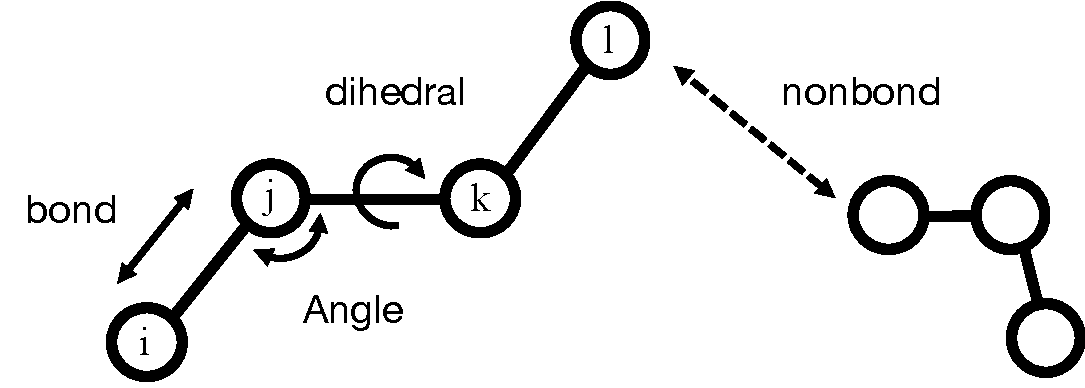
\includegraphics[width=0.5\hsize]{fig_biomol_model.pdf}
  \caption{生体分子の相互作用の模式図.}
  \label{Fig:BioModel}
 \end{center}
\end{figure}

\clearpage
\section{様々なポテンシャル関数: 力・ヴィリアルの表式}
この章では, 様々なポテンシャル関数を詳しく見ている.
また分子動力学シミュレーションの時間積分に必要な力や圧力計算に必要となるヴィリアルの
表式を解説する.
このノートでは位置ベクトルとして$\bm{r}_{ij} = \bm{r}_{j} - \bm{r}_{i}$の定義を使用する.

\subsection{結合長ポテンシャル: 調和振動子型}
\paragraph{結合長ポテンシャル}  \

共有結合をしている2原子間の相互作用は, 調和振動子で近似したポテンシャル関数
\begin{equation}
 U_{\mathrm{bond}}(r_{ij}) = k_{r} (r_{ij} - r_{\mathrm{eq}})^{2}
 \label{eq:BioModel2}
\end{equation}
を用いる. 
ここで, $k_{r}$はばね定数, $r_{ij}$は原子$i$と原子$j$の距離, $r_{\mathrm{eq}}$は平衡結合距離である.

\paragraph{結合長ポテンシャルの力} \

結合長による力は以下のように計算される:
\begin{alignat}{3}
    \bm{F}_{i}^{\mathrm{bond}}
 &= 
     -\frac{d U_{\mathrm{bond}}(r_{ij})}{d \bm{r}_{i}}
 &&= &
     2 k_{r} (r_{ij} - r_{\mathrm{eq}}) \frac{\bm{r}_{ij}}{r_{ij}}
 \label{eq:BioModel3}
 \\
 \bm{F}_{j}^{\mathrm{bond}}
 &=
   -\frac{d U_{\mathrm{bond}}(r_{ij})}{d \bm{r}_{j}}
 &&= -&
     2 k_{r} (r_{ij} - r_{\mathrm{eq}}) \frac{\bm{r}_{ij}}{r_{ij}}
 \label{eq:BioModel4}
\end{alignat}
ここで, 
\begin{equation}
 \bm{r}_{ij} = \bm{r}_{j} - \bm{r}_{i}
 \label{eq:BioModel4.5}
\end{equation}
とした.

\paragraph{結合長ポテンシャルのヴィリアル} \

ヴィリアルは
\begin{equation}
  -\left\langle
   \sum_{i=1}^{N} \bm{r}_{i}
   \cdot \frac{\partial U(\bm{r})}{\partial \bm{r}_{i}}
   \right\rangle
=
   \left\langle
   \sum_{i=1}^{N} \bm{r}_{i}
   \cdot \bm{F}_{i}
   \right\rangle
 \label{eq:BioModel5}
\end{equation}
で定義される. したがって, 結合長ポテンシャルに由来するヴィリアルは
\begin{align}
 \left\langle
   \sum_{i=1}^{N} \bm{r}_{i}
   \cdot \bm{F}_{i}
 \right\rangle
 &=
 \left\langle
   \sum_{\mathrm{bonds}}
   \left(
     \bm{r}_{i} \cdot \bm{F}_{i}^{\mathrm{bond}}
   + \bm{r}_{j} \cdot \bm{F}_{j}^{\mathrm{bond}}
 \right)
 \right\rangle
 \\
  &=
 \left\langle
   \sum_{\mathrm{bonds}}
   \left(
     \bm{r}_{ij} \cdot \bm{F}_{j}^{\mathrm{bond}}
 \right)
 \right\rangle
 \\
 &=
 \left\langle
      -\sum_{\mathrm{bonds}} 2 k_{r} (r_{ij} - r_{\mathrm{eq}}) r_{ij}
 \right\rangle
 \label{eq:BioModel6}
\end{align}
と計算される.

\clearpage

\subsection{結合長ポテンシャル: ガウス分布型}

\paragraph{ガウス分布型結合長ポテンシャル} \

共有結合をしている3つの原子$i,~j,~k$の結合角ポテンシャルを$i,~k$原子間の結合の相互作用として表すときにガウス分布型のポテンシャル関数

\begin{equation}
   U_{\mathrm{gauss}} (r_{ij})
   =
   \epsilon
   e^{-\frac{1}{2\sigma^{2}}(r_{ij} - r_{0})^{2}}
\end{equation}
を用いることがある. ここで, $r_{ij}$は原子$i$と原子$j$の距離, $r_{0}$は平行結合距離, $\epsilon$はポテンシャルの深さ, $\sigma$はポテンシャルの幅を表す.

\paragraph{ガウス分布型結合長ポテンシャルの力} \

ガウス分布型結合長ポテンシャルの力は以下のように計算される:

\begin{alignat}{3}
   \bm{F}_{i}^{\mathrm{gauss}}
   &=
   -&&
   \frac{\epsilon}{\sigma^{2}}
   (r_{ij} - r_{0})
   \cdot
   e^{-\frac{1}{2\sigma^{2}}(r_{ij} - r_{0})^{2}}
   \frac{\bm{r}_{ij}}{r_{ij}}
   \\
   \bm{F}_{j}^{\mathrm{gauss}}
   &=&&
   \frac{\epsilon}{\sigma^{2}}
   (r_{ij} - r_{0})
   \cdot
   e^{-\frac{1}{2\sigma^{2}}(r_{ij} - r_{0})^{2}}
   \frac{\bm{r}_{ij}}{r_{ij}}
\end{alignat}
ここで,
\begin{equation}
   \bm{r}_{ij} = \bm{r}_{j} - \bm{r}_{i}
\end{equation}
とした.


\paragraph{ガウス分布型結合長ポテンシャルのヴィリアル} \

ガウス分布型結合長ポテンシャルに由来するヴィリアルは
\begin{alignat}{3}
   \left\langle
      \bm{r}_{i} \cdot \bm{F}_{i}^{\mathrm{gauss}}
   \right\rangle
   =
   \left\langle
      \sum_{\mathrm{bonds}}
      \frac{\epsilon}{\sigma^{2}} r_{ij} (r_{ij} - r_{0})
      \cdot
      e^{-\frac{1}{2\sigma^{2}}(r_{ij} - r_{0})^{2}}
   \right\rangle
   \notag
\end{alignat}
と計算される.

\clearpage

\subsection{結合角ポテンシャル: 調和振動子型}
\paragraph{結合角ポテンシャル} \

共有結合をしている3つの原子間に関しては調和振動子で近似したポテンシャル関数
\begin{equation}
    U_{\mathrm{angle}}(\theta_{ijk})
  = k_{\theta} (\theta_{ijk} - \theta_{\mathrm{eq}})^{2}
 \label{eq:BioModel7}
\end{equation}
を用いる. ここで, $k_{\theta}$はばね定数, $\theta_{\mathrm{eq}}$は平衡結合角, 
$\theta_{ijk}$は結合角である. 
また, 
\begin{align}
  &\bm{r}_{ji}
 = \bm{r}_{i} - \bm{r}_{j}
 \label{eq:BioModel8}
 \\
  &\bm{r}_{jk}
 = \bm{r}_{k} - \bm{r}_{j}
 \label{eq:BioModel9}
 \\
  &\theta_{ijk}
 = \arccos \left(
                  \frac{\bm{r}_{ji} \cdot \bm{r}_{jk}}{r_{ji} r_{jk}}
           \right)
 \label{eq:BioModel10}
\end{align}
と定義した.

\paragraph{結合角ポテンシャルの力} \

 結合角による力は以下のように計算される:
\begin{alignat}{3}
     \bm{F}_{i}^{\mathrm{angle}}
 &= 
    -\frac{d U_{\mathrm{angle}}(\theta_{ijk})}{d \bm{r}_{i}}
 &&=
     2k_{\theta} (\theta_{ijk} - \theta_{\mathrm{eq}})
     \frac{1}{r_{ji} \sin \theta_{ijk}}
     \left(
            \frac{\bm{r}_{jk}}{r_{jk}} - \cos \theta_{ijk} \frac{\bm{r}_{ji}}{r_{ji}}
     \right)
 \label{eq:BioModel11}
 \\
     \bm{F}_{k}^{\mathrm{angle}}
 &= 
    -\frac{d U_{\mathrm{angle}}(\theta_{ijk})}{d \bm{r}_{k}}
 &&=
    2k_{\theta} (\theta_{ijk} - \theta_{\mathrm{eq}})
    \frac{1}{r_{jk} \sin \theta_{ijk}}
    \left(
           \frac{\bm{r}_{ji}}{r_{ji}} - \cos \theta_{ijk} \frac{\bm{r}_{jk}}{r_{jk}}
    \right)
 \label{eq:BioModel12}
 \\
     \bm{F}_{j}^{\mathrm{angle}}
 &= 
    -\frac{d U_{\mathrm{angle}}(\theta_{ijk})}{d \bm{r}_{j}}
 &&=
    -\bm{F}_{i}^{\mathrm{angle}} - \bm{F}_{k}^{\mathrm{angle}}
 \label{eq:BioModel13}
\end{alignat}

\paragraph{結合角ポテンシャルのヴィリアル} \

結合角ポテンシャルに由来するヴィリアルは, 
\begin{align}
    \bm{r}_{i} \cdot \bm{F}_{i}^{\mathrm{angle}}
   +\bm{r}_{j} \cdot \bm{F}_{j}^{\mathrm{angle}}
   +\bm{r}_{i} \cdot \bm{F}_{i}^{\mathrm{angle}}
 &=
    (\bm{r}_{i} - \bm{r}_{j}) \cdot \bm{F}_{i}^{\mathrm{angle}}
   +(\bm{r}_{k} - \bm{r}_{j}) \cdot \bm{F}_{k}^{\mathrm{angle}}
 \notag
 \\
 &=
    2k_{\theta} (\theta_{ijk} - \theta_{\mathrm{eq}}) \frac{1}{\sin \theta_{ijk}}
 \notag
 \\
 &~~~~ \times
    \left(
           \frac{\bm{r}_{ji} \cdot \bm{r}_{jk}}{r_{ji} r_{jk}} - \cos \theta_{ijk}
          +\frac{\bm{r}_{jk} \cdot \bm{r}_{ji}}{r_{jk} r_{ji}} - \cos \theta_{ijk}
    \right)
 \notag
 \\
 &=
    0
 \notag
\end{align}
であることからヴィリアルの値はゼロとなる. 

\clearpage

\subsection{角度に対するフィルター関数}

特定の角度周辺でのみポテンシャルを課すために, 次のようなフィルター関数をポテンシャル関数に乗じることがある:
\begin{align}
   f(K, \Delta \theta)
   =
   \begin{cases}
      1 &
      (\text{when}~\frac{-\pi}{2K} \le \Delta \theta \le \frac{\pi}{2K})\\
      1 - \cos^{2} (K \Delta \theta) &
      (\text{when}~\frac{-\pi}{K} < \Delta \theta < \frac{-\pi}{2K}~
       \text{or}~  \frac{\pi}{2K} < \Delta \theta < \frac{\pi}{K}) \\
      0 &
      (\text{when}~ \Delta \theta \le \frac{-\pi}{K}~
       \text{or}~ \Delta \theta \ge \frac{\pi}{K})
   \end{cases}
\end{align}
ここで, $K$はフィルター関数の幅を指定するパラメータ, $\Delta \theta = \theta_{ijk} - \theta_{0}$は目的の角度$\theta_{0}$からのずれである.
目的の角度周辺では1, 離れた領域では0, そしてそれらの領域の間を滑らかに繋いだ, 丘のような形をした関数となっている. なお, ここでは角度を
\begin{align}
   \bm{r}_{ji}
   &= \bm{r}_{i} - \bm{r}_{j}
   \\
   \bm{r}_{jk}
   &= \bm{r}_{k} - \bm{r}_{j}
   \notag \\
    \theta_{ijk}
   &= \arccos \left( \frac{\bm{r}_{ji} \cdot \bm{r}_{jk}}{r_{ji} r_{jk}} \right)
   \\
   \cos(\theta_{ijk})
   &= \frac{\bm{r}_{ji} \cdot \bm{r}_{jk}}{r_{ji} r_{jk}}
   = \frac{(\bm{r}_{i} - \bm{r}_{j}) \cdot (\bm{r}_{k} - \bm{r}_{j})}
         {\left\{(\bm{r}_{i} - \bm{r}_{j})\right\}^{\frac{1}{2}}
          \left\{(\bm{r}_{k} - \bm{r}_{j})\right\}^{\frac{1}{2}}}
\end{align}
と定義する.

\paragraph{フィルター関数に由来する力} \

フィルター関数に由来する力は
\begin{align}
   \bm{F}_{i}^{\mathrm{filter}}
   &=
   \frac{2K \sin (2K \Delta \theta)}{r_{ji} \sin\theta_{ijk}}
   \left(
            \frac{\bm{r}_{jk}}{r_{jk}}
          - \cos\theta_{ijk} \frac{\bm{r}_{ji}}{r_{ji}}
   \right)
   \\
   \bm{F}_{k}^{\mathrm{filter}}
   &=
   \frac{2K \sin (2K \Delta \theta)}{r_{jk} \sin\theta_{ijk}}
   \left(
           \frac{\bm{r}_{ji}}{r_{ji}}
         - \cos\theta_{ijk} \frac{\bm{r}_{jk}}{r_{jk}}
   \right)
   \\
   \bm{F}_{j}^{\mathrm{filter}}
   &=
   - \bm{F}_{i}^{\mathrm{filter}} - \bm{F}_{k}^{\mathrm{filter}}
\end{align}
のように計算することができる.



\clearpage
\subsection{二面角ポテンシャル: フーリエ級数型}
\paragraph{二面角ポテンシャル} \

共有結合した4原子が作る二面角に対するポテンシャルを,
\begin{equation}
    U_{\mathrm{dihedral}}(\phi_{ijkl})
  =
    \frac{V}{2} [1 + \cos(n\phi_{ijkl} - \gamma)]
 \label{eq:BioModel14}
\end{equation}
で表すことができる.
ここで, $V$はエネルギーバリア, $n$は周期, $\gamma$は位相である. 二面角$\phi_{ijkl}$は
\begin{alignat}{2}
 &\bm{r}_{ji} &&= \bm{r}_{i} - \bm{r}_{j}
 \label{eq:BioModel15}
 \\
 &\bm{r}_{kj} &&= \bm{r}_{j} - \bm{r}_{k}
 \label{eq:BioModel16}
 \\
 &\bm{r}_{lk} &&= \bm{r}_{k} - \bm{r}_{l}
 \label{eq:BioModel17}
 \\
 &\bm{n}_{j}  &&= \bm{r}_{ji} \times \bm{r}_{jk}
 \label{eq:BioModel18}
 \\
 &\bm{n}_{k}  &&= \bm{r}_{kj} \times \bm{r}_{kl}
 \label{eq:BioModel19}
 \\
 &\phi_{ijkl} &&=
 - \mathrm{sign}
   \left[
         \arccos \left( \frac{\bm{n}_{j} \cdot \bm{n}_{k}}{n_{j} n_{k}}\right)
         ,~
         \bm{r}_{kj} \cdot \bm{n}_{j} \times \bm{n}_{k}
   \right]
 \label{eq:BioModel20}
\end{alignat}
で定義される. 
ただし, $\mathrm{sign}[a,b]$は$(\mathrm{bの符号}) \times (\mathrm{aの絶対値})$と計算される. 

\paragraph{二面角ポテンシャルの力} \

二面角による力は以下のように計算される:
\begin{alignat}{3}
     \bm{F}_{i}^{\mathrm{dihedral}}
 &=
    -\frac{d U_{\mathrm{dihedral}}(\phi_{ijkl})}{d \bm{r}_{i}}
 &&=
     f_{0} (\bm{r}_{kj} \times \bm{f}_{\mathrm{kj}})
 \label{eq:BioModel21}
 \\
     \bm{F}_{j}^{\mathrm{dihedral}}
 &=
    -\frac{d U_{\mathrm{dihedral}}(\phi_{ijkl})}{d \bm{r}_{j}}
 &&=
     f_{0}
     \left( \bm{r}_{lk} \times \bm{f}_{jk}
           -\bm{r}_{kj} \times \bm{f}_{kj}
           -\bm{r}_{ji} \times \bm{f}_{kj}
     \right)
 \label{eq:BioModel22}
 \\
     \bm{F}_{k}^{\mathrm{dihedral}}
 &=
    -\frac{d U_{\mathrm{dihedral}}(\phi_{ijkl})}{d \bm{r}_{k}}
 &&=
    f_{0}
    \left( \bm{r}_{ji} \times \bm{f}_{kj}
          -\bm{r}_{lk} \times \bm{f}_{jk}
          -\bm{r}_{kj} \times \bm{f}_{jk}
    \right)
 \label{eq:BioModel23}
 \\
 \bm{F}_{l}^{\mathrm{dihedral}}
 &=
     -\frac{d U_{\mathrm{dihedral}}(\phi_{ijkl})}{d \bm{r}_{l}}
 &&=
     f_{0} ( \bm{r}_{kj} \times \bm{f}_{jk} )
 \label{eq:BioModel24}
\end{alignat}
ただし, 
\begin{align}
 f_{0}
 &=
    \frac{nV}{2} \frac{\sin(n \phi - \gamma)}{\sin \phi}
 \label{eq:BioModel25}
 \\
 \bm{f}_{kj}
 &=
    \frac{1}{n_{j}}
    \left(
           \frac{\bm{n}_{k}}{n_{k}} - \cos \phi \frac{\bm{n}_{j}}{n_{j}}
    \right)
 \label{eq:BioModel26}
 \\
 \bm{f}_{jk}
 &=
    \frac{1}{n_{k}}
    \left(
          \frac{\bm{n}_{j}}{n_{j}} - \cos \phi \frac{\bm{n}_{k}}{n_{k}}
    \right)
 \label{eq:BioModel27}
\end{align}
である. $\bm{f}_{\alpha}$($\alpha = 1, 2, 3, 4$)を
\begin{align}
 \bm{f}_{1} &= f_{0} ( \bm{r}_{kj} \times \bm{f}_{kj}) \\
 \bm{f}_{2} &= f_{0} ( \bm{r}_{lk} \times \bm{f}_{jk}) \\
 \bm{f}_{3} &= f_{0} ( \bm{r}_{ji} \times \bm{f}_{kj}) \\
 \bm{f}_{4} &= f_{0} ( \bm{r}_{kj} \times \bm{f}_{jk})
\end{align}
のように定義すると, 二面角による力は
\begin{align}
 \bm{F}_{i}^{\mathrm{dihedral}} &= \bm{f}_{1} \\
 \bm{F}_{j}^{\mathrm{dihedral}} &= \bm{f}_{2} - \bm{f}_{1} - \bm{f}_{3} \\
 \bm{F}_{k}^{\mathrm{dihedral}} &= \bm{f}_{3} - \bm{f}_{2} - \bm{f}_{4} \\
 \bm{F}_{l}^{\mathrm{dihedral}} &= \bm{f}_{4}
\end{align}
と書くことができる. 
 
\paragraph{二面角ポテンシャルのヴィリアル} \

ベクトル三重積の公式
\begin{align}
   \bm{A} \times (\bm{B} \times \bm{C})
 =
   (\bm{A} \cdot \bm{C}) \bm{B}
  -(\bm{A} \cdot \bm{B}) \bm{C}
\end{align}
を用いると, $\bm{f}_{kj}$と$\bm{f}_{jk}$は
\begin{align}
    \bm{f}_{kj}
 &=
    \frac{1}{n_{j}^{3} n_{k}}
    \left\{
            \bm{n}_{j} \times (\bm{n}_{k} \times \bm{n}_{j})
     \right\}
 \\
    \bm{f}_{jk}
 &=
    \frac{1}{n_{j} n_{k}^{3}}
    \left\{
            \bm{n}_{k} \times (\bm{n}_{j} \times \bm{n}_{k})
    \right\}
\end{align}
と書き直せる. さらに, 右辺に2つある$\bm{n}_{j}$あるいは$\bm{n}_k$に定義式(\ref{eq:BioModel18}), (\ref{eq:BioModel19})を代入して, 
ベクトル三重積の公式を繰り返し適用させると, 
\begin{align}
    \bm{n}_{j} \times (\bm{n}_{k} \times \bm{n}_{j})
 &=
   -(\bm{n}_{k} \cdot \bm{r}_{ji})
    \left\{
            (\bm{r}_{jk} \cdot \bm{r}_{jk})\bm{r}_{ji}
           -(\bm{r}_{jk} \cdot \bm{r}_{ji})\bm{r}_{jk}
    \right\}
 \\
    \bm{n}_{k} \times (\bm{n}_{j} \times \bm{n}_{k})
 &=
   -(\bm{n}_{j} \cdot \bm{r}_{kl})
    \left\{
            (\bm{r}_{kj} \cdot \bm{r}_{kl})\bm{r}_{kj}
           -(\bm{r}_{kj} \cdot \bm{r}_{kj})\bm{r}_{kl}
    \right\}
\end{align}
が得られ, 
\begin{align}
    \bm{f}_{1}
 &= 
    \frac{f_{0}}{n_{j}^{3}n_{k}}
    (\bm{n}_{k} \cdot \bm{r}_{ji})
    (\bm{r}_{jk} \cdot \bm{r}_{jk})
    (\bm{r}_{kj} \times \bm{r}_{ji})
 \\
    \bm{f}_{2}
 &= 
    \frac{-f_{0}}{n_{j}n_{k}^{3}}
    (\bm{n}_{j} \cdot \bm{r}_{kl})
    (\bm{r}_{kj} \cdot \bm{r}_{kl})
    (\bm{r}_{lk} \times \bm{r}_{kj})
 \\
    \bm{f}_{3}
 &= 
    \frac{-f_{0}}{n_{j}^{3}n_{k}}
    (\bm{n}_{k} \cdot \bm{r}_{ji})
    (\bm{r}_{jk} \cdot \bm{r}_{ji})
    (\bm{r}_{ji} \times \bm{r}_{jk})
 \\
    \bm{f}_{3}
 &= 
    \frac{f_{0}}{n_{j}n_{k}^{3}}
    (\bm{n}_{j} \cdot \bm{r}_{kl})
    (\bm{r}_{kj} \cdot \bm{r}_{kj})
    (\bm{r}_{kj} \times \bm{r}_{kl})
\end{align}
と計算される. これらを用いると,
\begin{align}
   \bm{r}_{i} \cdot \bm{F}_{i}^{\mathrm{dihedral}}
 + \bm{r}_{j} \cdot \bm{F}_{j}^{\mathrm{dihedral}}
 + \bm{r}_{k} \cdot \bm{F}_{k}^{\mathrm{dihedral}}
 + \bm{r}_{l} \cdot \bm{F}_{l}^{\mathrm{dihedral}}
 = 0
\end{align}
となることが確認できるため, 二面角ポテンシャルに由来するヴィリアルはゼロとなる. 

\clearpage

\subsection{二面角ポテンシャル: ガウス分布型}

\paragraph{ガウス分布型二面角ポテンシャル} \

共有結合をしている3つの原子$i,~j,~k,~l$の二面角ポテンシャルをガウス分布型のポテンシャル関数
\begin{equation}
   U_{\mathrm{gauss}} (\phi_{ijkl})
   =
   \epsilon
   e^{-\frac{1}{2\sigma^{2}}(\phi_{ijkl} - \phi_{0})^{2}}
\end{equation}
を用いて表すことがある. ここで, $r_{ij}$は原子$i$と原子$j$の距離, $r_{0}$は平行結合距離, $\epsilon$はポテンシャルの深さ, $\sigma$はポテンシャルの幅を表す. ここで二面角は
\begin{alignat}{1}
   \bm{r}_{ji} &= \bm{r}_{i} - \bm{r}_{j}
   \notag \\
   \bm{r}_{kj} &= \bm{r}_{j} - \bm{r}_{k}
   \notag \\
   \bm{r}_{lk} &= \bm{r}_{k} - \bm{r}_{l}
   \notag \\
   \bm{n}_{j}  &= \bm{r}_{ji} \times \bm{r}_{jk}
   \notag \\
   \bm{n}_{k}  &= \bm{r}_{kj} \times \bm{r}_{kl}
   \notag
   \\
   \phi_{ijkl} &=
   - \mathrm{sign}
     \left[
           \arccos \left( \frac{\bm{n}_{j} \cdot \bm{n}_{k}}{n_{j} n_{k}}\right),
           \bm{r}_{kj} \cdot \bm{n}_{j} \times \bm{n}_{k}
     \right]
   \notag
\end{alignat}
と定義する.

\paragraph{ガウス分布型二面角ポテンシャルの力} \

ガウス分布型二面角ポテンシャルの力は係数を除いて, フーリエ級数型ポテンシャルと同じように計算することができる.
すなわち, 
\begin{align}
   f_{0}
   &\equiv
   \frac{\epsilon(\phi_{ijkl} - \phi_{0})}{\sigma^{2} \sin \phi_{ijkl}}
   e^{-\frac{1}{2\sigma^{2}}(\phi_{ijkl} - \phi_{0})^{2}}
   \\
   \bm{f}_{kj}
   &\equiv
   \left\{
      \frac{1}{n_{j}}
      \left(
             \frac{\bm{n}_{k}}{n_{k}} - \cos\phi \frac{\bm{n}_{j}}{n_{j}}
      \right)
   \right\}
   \\
   \bm{f}_{jk}
   &\equiv
   \left\{
      \frac{1}{n_{k}}
      \left(
             \frac{\bm{n}_{j}}{n_{j}} - \cos\phi \frac{\bm{n}_{k}}{n_{k}}
      \right)
   \right\}
\end{align}
と置いた時に, 各粒子に加わる力は
\begin{alignat}{5}
   \bm{F}_{i}
   &=
   &&
   f_{0} (\bm{r}_{kj} \times \bm{f}_{kj})
   \\
   \bm{F}_{j}
   &=
   &&
   f_{0} (\bm{r}_{lk} \times \bm{f}_{jk} - \bm{r}_{ki} \times \bm{f}_{kj})
   &=
   f_{0}
   ( \bm{r}_{lk} \times \bm{f}_{jk}
   - \bm{r}_{kj} \times \bm{f}_{kj}
   - \bm{r}_{ji} \times \bm{f}_{kj} )
   \\
   \bm{F}_{k}
   &=&&
   f_{0} (\bm{r}_{ji} \times \bm{f}_{kj} - \bm{r}_{lj} \times \bm{f}_{jk})
   &=
   f_{0}
   ( \bm{r}_{ji} \times \bm{f}_{kj}
   - \bm{r}_{lk} \times \bm{f}_{jk}
   - \bm{r}_{kj} \times \bm{f}_{jk})
   \\
   \bm{F}_{l}
   &=&&
   f_{0} (\bm{r}_{kj} \times \bm{f}_{jk})
\end{alignat}
と計算できる.


\paragraph{ガウス分布型二面角ポテンシャルのヴィリアル} \

ガウス分布型二面角ポテンシャルの力の表式が, 係数$f_{0}$を除いてフーリエ級数型の二面角ポテンシャルと同じであることに注目すると, フーリエ級数型の二面角ポテンシャルの時と同様の計算によって
\begin{align}
   \bm{r}_{i} \cdot \bm{F}_{i}^{\mathrm{dihedral}}
 + \bm{r}_{j} \cdot \bm{F}_{j}^{\mathrm{dihedral}}
 + \bm{r}_{k} \cdot \bm{F}_{k}^{\mathrm{dihedral}}
 + \bm{r}_{l} \cdot \bm{F}_{l}^{\mathrm{dihedral}}
 = 0
\end{align}
となることが確認できる. すなわち, ガウス分布型二面角ポテンシャルのヴィリアルはゼロとなる.

\clearpage
\subsection{ファンデル・ワールス相互作用: 12-6型}
\paragraph{ファンデル・ワールス相互作用} \

ファンデル・ワールス相互作用によるポテンシャルは, レナード・ジョーンズポテンシャル用いて
\begin{equation}
    U_{\mathrm{LJ}}(r_{ij})
 =
   4\epsilon_{ij}
   \left\{
           \left(\frac{\sigma_{ij}}{r_{ij}}\right)^{12}
          -\left(\frac{\sigma_{ij}}{r_{ij}}\right)^{6}
   \right\}
 \label{eq:BioModel29}
\end{equation}
と与えられる.
ここで, $\epsilon_{ij}$はポテンシャルの深さ, $\sigma_{ij}$は粒子間の最小相互作用距離, 
$r_{ij}$は粒子間の距離を表している. 
第1項目は電子雲の重なりに起因する反発項, 第2項目は分散力に起因する引力項である. 
$\epsilon_{ij}$と$\sigma_{ij}$はローレンツ・ベルテロー則を用いて
各原子についてのポテンシャルの深さ$\epsilon_{i}$と粒子の直径$\sigma_{i}$から
\begin{align}
 \epsilon_{ij} &= \sqrt{\epsilon_{i} \epsilon_{j}}
 \\
 \sigma  _{ij} &= \frac{\sigma_{i} + \sigma_{j}}{2}
 \label{eq:BioModel30}
\end{align}
で与えられることが多い.
LJ相互作用の計算は$\mathcal{O}(N^2)$となり計算コストがかかる. 
しかし, 収束の速い関数であるため通常はカットオフを設定し, カットオフ半径内に存在する粒子対のみ計算することで
計算コストを抑えることができる. 
カットオフ半径$r_{c}$は系のボックスサイズの半分以下の大きさの値に設定する. 

\paragraph{ファンデル・ワールス相互作用の力} \

レナード・ジョーンズ相互作用による力は以下のように計算される:
\begin{alignat}{3}
    \bm{F}_{i}^{\mathrm{LJ}}
 &=
   -\frac{d U_{\mathrm{LJ}}(r_{ij})}{d \bm{r}_{i}}
  =
   -&&
   24 \epsilon_{ij}
   \left\{
           2\left( \frac{\sigma_{ij}}{r_{ij}} \right)^{12}
          - \left( \frac{\sigma_{ij}}{r_{ij}} \right)^{6}
   \right\}
   \frac{\bm{r}_{ij}}{r_{ij}^{2}}
 \label{eq:BioModel31}
 \\
    \bm{F}_{j}^{\mathrm{LJ}}
 &=
   -\frac{d U_{\mathrm{LJ}}(r_{ij})}{d \bm{r}_{j}}
 =
   &&
   24 \epsilon_{ij}
   \left\{
           2\left( \frac{\sigma_{ij}}{r_{ij}} \right)^{12}
          - \left( \frac{\sigma_{ij}}{r_{ij}} \right)^{6}
   \right\}
   \frac{\bm{r}_{ij}}{r_{ij}^{2}}
 \label{eq:BioModel32}
\end{alignat}

\paragraph{ファンデル・ワールス相互作用のヴィリアル} \

ファンデル・ワールス相互作用に由来するヴィリアルは, 
\begin{align}
 &\left\langle
  \sum_{i=1}^{N} \sum_{j > i}^{N}
  24 \epsilon_{ij}
  \left\{
        2 \left( \frac{\sigma_{ij}}{r_{ij}} \right)^{12}
        - \left( \frac{\sigma_{ij}}{r_{ij}} \right)^{6}
  \right\}
 \right\rangle
 \\
 =
  &\left\langle
   \sum_{\mathrm{nonbonds}}
   24 \epsilon_{ij}
   \left\{
           2\left( \frac{\sigma_{ij}}{r_{ij}} \right)^{12}
          - \left( \frac{\sigma_{ij}}{r_{ij}} \right)^{6}
   \right\}
   \right\rangle
 \label{eq:BioModel33}
\end{align}
で計算される. 

\clearpage

\subsection{モースポテンシャル}
\paragraph{モースポテンシャル} \

モースポテンシャルは2原子の結合・解離を記述するときに使用されるポテンシャルである.
具体的なポテンシャル関数は,

\begin{equation}
   U_{\mathrm{morse}} (r_{ij})
   =
   \epsilon
   \left\{
      1 - e^{-\alpha(r_{ij} - r_{0})}
   \right\}^{2}
\end{equation}
とかける. ここで, $r_{ij}$は2原子間の距離, $\epsilon$はポテンシャルの深さ, $\alpha$はポテンシャルの幅, $r_{i}$は2原子の平衡結合距離を表す.

\paragraph{モースポテンシャルによる力} \

モースポテンシャルによって原子がうける力は以下のように計算される.
\begin{alignat}{3}
   \bm{F}_{i}^{\mathrm{morse}}
   =
   -
   \frac{d U_{\mathrm{morse}}(r_{ij})}{d \bm{r}_{i}}
   &=&&
   2\epsilon \alpha
   \left\{
      e^{-\alpha(r_{ij} - r_{0})}
      -
      e^{-2\alpha(r_{ij} - r_{0})}
   \right\}
   \frac{\bm{r}_{ij}}{r_{ij}}
   \\
   \bm{F}_{j}^{\mathrm{morse}}
   =
   -
   \frac{d U_{\mathrm{morse}}(r_{ij})}{d \bm{r}_{j}}
   &=
   -&&
   2\epsilon \alpha
   \left\{
      e^{-\alpha(r_{ij} - r_{0})}
      -
      e^{-2\alpha(r_{ij} - r_{0})}
   \right\}
   \frac{\bm{r}_{ij}}{r_{ij}}
\end{alignat}
ただし,
\begin{align}
   \bm{r}_{ij} = \bm{r}_{j} - \bm{r}_{i}
\end{align}
と定義した.

\paragraph{モースポテンシャルに由来するヴィリアル} \

モースポテンシャル相互作用に由来するヴィリアルは, 
\begin{align}
   \left\langle
        \sum_{i=1}^{N} \bm{r}_{i} \cdot \bm{F}_{i}^{\mathrm{morse}}
   \right\rangle
 =
   \left\langle
        \sum_{\mathrm{nonbonds}}
        -2\epsilon \alpha r_{ij}
        \left\{
           e^{-\alpha(r_{ij} - r_{0})}
           -
           e^{-2\alpha(r_{ij} - r_{0})}
        \right\}
   \right\rangle
\end{align}
と計算できる.

\clearpage

\subsection{静電相互作用}
\paragraph{静電ポテンシャル} \

電磁気でよく知られるように静電ポテンシャルは

\begin{equation}
U_{\mathrm{elec}}(r_{ij}) = \frac{q_{i}q_{j}}{4 \pi \epsilon_{0}}
                            \frac{1}{r_{ij}}
\end{equation}
とかける.
$q_{i}$と$q_{j}$はそれぞれ原子$i$と原子$j$の電荷, $\epsilon_{0}$は真空中の誘電率, 
$r_{ij}$は原子$i$と原子$j$の距離である.

静電相互作用はレナードジョーンズ相互作用と比較して, 減衰が遅いポテンシャル関数である.
そのため計算コストを減少するためのカットオフをしてしまうと誤差を生み出す原因となる.
このような問題を回避するための方法として, Ewald法やParticle Mesh Ewald法,
多極子展開法など様々な取扱方法がこれまでに提案されてきている\cite{2014Cisneros}.

\paragraph{静電ポテンシャルによる力} \

静電相互作用による力は以下のように計算される.
\begin{alignat}{3}
   \bm{F}_{i}^{\mathrm{elec}}
 &=
   -\frac{d U_{\mathrm{elec}}(r_{ij})}{d \bm{r}_{i}}
&&=&
   -\frac{q_{i}q_{j}}{4 \pi \epsilon_{0} r_{ij}^{2}}
    \frac{\bm{r}_{ij}}{r_{ij}}
 \\
    \bm{F}_{j}^{\mathrm{elec}}
 &=
   -\frac{d U_{\mathrm{elec}}(r_{ij})}{d \bm{r}_{j}}
&&=&
    \frac{q_{i}q_{j}}{4 \pi \epsilon_{0} r_{ij}^{2}}
    \frac{\bm{r}_{ij}}{r_{ij}}
 \\
\end{alignat}

\paragraph{静電ポテンシャルによるヴィリアル} \

静電相互作用に由来するヴィリアルは,
\begin{align}
  \left\langle
  \sum_{i=1}^{N} \sum_{j > i}^{N}
  \frac{q_{i}q_{j}}{4 \pi \epsilon_{0}}
  \frac{1}{r_{ij}}
  \right\rangle
 =
  \left\langle
  \sum_{\mathrm{nonbonds}}
  \frac{q_{i}q_{j}}{4 \pi \epsilon_{0}}
  \frac{1}{r_{ij}}
  \right\rangle
\end{align}
となる.

\clearpage
\section{計算ノート: 微分・力・ヴィリアルの導出}
\subsection{力の計算の基本的な手順}
粒子$\alpha$に加わる力は, ポテンシャルを座標ベクトル$\bm{r}_{\alpha}$に関して微分すれば良い. すなわち

\begin{align}
   \bm{F}_{\alpha}
   =
   -
   \frac{d U}{d \bm{r}_{\alpha}}
\end{align}
と計算できる.
代表的なポテンシャル関数として(1)調和振動子, (2)ガウス関数, (3) フーリエ級数 ($\cos$関数, $\sin$関数), (4) レナード・ジョーンズポテンシャル, (5) モースポテンシャル, (6)静電相互作用がある.
さらに, 多くの場合でポテンシャル関数は内部座標を用いて表されることが多い.
例えば, 2体相互作用であれば, 2点間の距離$r_{ij}$, 3体相互作用であれば, 3点間の角度$\theta_{ijk}$, 4体相互作用であれば4点間の二面角$\phi_{ijkl}$の関数で表されることが多い.

微分の連鎖率を用いると, 力の計算は(i)ポテンシャルの変数に関する微分, (ii)ポテンシャルの変数の座標ベクトル微分の積で書くことができる. すなわち
\begin{align}
   \bm{F}_{\alpha}
   =
   -
   \frac{d U}{d \lambda}
   \frac{d \lambda}{d \bm{r}_{\alpha}}
\end{align}
となる. 第1項目はポテンシャル関数形ごとに計算される項である. 第2項目は内部座標に依存する項で, 力の向きに関係してくる.


\subsection{2点間の距離$r_{ij}$を粒子の位置ベクトル$\bm{r}_{\alpha}$で微分する}
\subsubsection{ベクトルの定義}
質点の位置$\bm{r}_{i}$から$\bm{r}_{j}$に向かうベクトルを
\begin{align}
   \bm{r}_{ij}
&= \bm{r}_{j} - \bm{r}_{i}
\end{align}
と定義する. 2点間の距離は
\begin{align}
   r_{ij} = \left(\bm{r}_{ij} \cdot \bm{r}_{ij} \right)^{\frac{1}{2}}
\end{align}
と計算される.
\subsubsection{座標ベクトル微分の計算}
\begin{align}
\frac{d r_{ij}}{d \bm{r}_{i}}
&=
\left[
   \frac{d}{d \bm{r}_{i}}
   \left\{ (\bm{r}_{j} - \bm{r}_{i} )^{2} \right\}^{\frac{1}{2}}
\right]
=
\frac{1}{2}
\frac{ -2 (\bm{r}_{j} - \bm{r}_{i}) }
     { \left\{ ( \bm{r}_{j} - \bm{r}_{i} )^{2} \right\}^{\frac{1}{2}} }
=
-
\frac{\bm{r}_{ij}}{r_{ij}}
\label{Eq:dr_ij-dr_i}
\\
\frac{d r_{ij}}{d \bm{r}_{j}}
&=
\left[
   \frac{d}{d \bm{r}_{j}}
   \left\{ (\bm{r}_{j} - \bm{r}_{i} )^{2} \right\}^{\frac{1}{2}}
\right]
=
\frac{1}{2}
\frac{ 2 (\bm{r}_{j} - \bm{r}_{i}) }
     { \left\{ ( \bm{r}_{j} - \bm{r}_{i} )^{2} \right\}^{\frac{1}{2}} }
=
\frac{\bm{r}_{ij}}{r_{ij}}
\label{Eq:dr_ij-dr_j}
\end{align}

\subsection{3点間の角度$\theta_{ijk}$を粒子の位置ベクトル$\bm{r}_{\alpha}$で微分する}
\subsubsection{ベクトルと角度の定義}
3点間の角度$\theta_{ijk}$を
\begin{align}
   \bm{r}_{ji}
&= \bm{r}_{i} - \bm{r}_{j}
\\
   \bm{r}_{jk}
&= \bm{r}_{k} - \bm{r}_{j}
\\
   \theta_{ijk}
&= \arccos \left( \frac{\bm{r}_{ji} \cdot \bm{r}_{jk}}{r_{ji} r_{jk}} \right)
\\
   \cos(\theta_{ijk})
&= \frac{\bm{r}_{ji} \cdot \bm{r}_{jk}}{r_{ji} r_{jk}}
 = \frac{(\bm{r}_{i} - \bm{r}_{j}) \cdot (\bm{r}_{k} - \bm{r}_{j})}
        {\left\{(\bm{r}_{i} - \bm{r}_{j})\right\}^{\frac{1}{2}}
         \left\{(\bm{r}_{k} - \bm{r}_{j})\right\}^{\frac{1}{2}}}
\end{align}
と定義する.

\subsubsection{座標ベクトル微分の計算}
3点間の角度$\theta_{ijk}$を粒子の位置ベクトル$\bm{r}_{\alpha}$で微分すると
\begin{align}
    \frac{d \theta_{ijk}}{d \bm{r}_{\alpha}}
 &=
    \frac{d}{d \bm{r}_{\alpha}}
    \arccos \left( \frac{\bm{r}_{ji} \cdot \bm{r}_{jk}}{r_{ji} r_{jk}} \right)
 \notag \\
 &=
   -\frac{1}
         {\sqrt{1- \left(\frac{\bm{r}_{ji} \cdot \bm{r}_{jk}}{r_{ji} r_{jk}}\right)^{2}}}
    \left\{
            \frac{d}{d \bm{r}_{\alpha}}
            \left(\frac{\bm{r}_{ji} \cdot \bm{r}_{jk}}{r_{ji} r_{jk}}\right)
    \right\}
 \notag \\
 &=
   -\frac{1}{\sin\theta_{ijk}}
    \left\{
            \frac{d}{d \bm{r}_{\alpha}}
            \left(\frac{\bm{r}_{ji} \cdot \bm{r}_{jk}}{r_{ji} r_{jk}}\right)
    \right\}
  \notag
\end{align}
を得る. 第2式から第3式において, $\arccos(x)$の微分公式
\begin{equation}
\frac{d}{dx}\arccos(x) = - \frac{1}{\sqrt{1-x^2}}
\notag
\end{equation}
を用いた. 続いて
\begin{equation}
 \frac{d}{d \bm{r}_{\alpha}}
 \left(\frac{\bm{r}_{ji} \cdot \bm{r}_{jk}}{r_{ji} r_{jk}}\right)
 \notag
\end{equation}
を各粒子$i$,$j$,$k$について計算していく.

\paragraph{$\alpha = i$のとき}
\begin{align}
    \frac{d}{d \bm{r}_{i}}
    \left(\frac{\bm{r}_{ji} \cdot \bm{r}_{jk}}{r_{ji} r_{jk}}\right)
 &=
    \frac{d}{d \bm{r}_{i}}
    \left[\frac{(\bm{r}_{i} - \bm{r}_{j}) \cdot (\bm{r}_{k} - \bm{r}_{j})}
               {\left\{ (\bm{r}_{i} - \bm{r}_{j})^{2} \right\}^{\frac{1}{2}}
                \left\{ (\bm{r}_{k} - \bm{r}_{j})^{2} \right\}^{\frac{1}{2}}}
    \right]
 \notag \\
 &=
    \frac{d}{d \bm{r}_{i}}
    \left[(\bm{r}_{i} - \bm{r}_{j}) \cdot (\bm{r}_{k} - \bm{r}_{j})
           \left\{ (\bm{r}_{i} - \bm{r}_{j})^{2} \right\}^{-\frac{1}{2}}
           \left\{ (\bm{r}_{k} - \bm{r}_{j})^{2} \right\}^{-\frac{1}{2}}
    \right]
 \notag \\
 &=
     \frac{(\bm{r}_{k} - \bm{r}_{j})}{r_{ji} r_{jk}}
   - \frac{1}{2}
     \frac{2(\bm{r}_{i} - \bm{r}_{j})
           \{(\bm{r}_{i} - \bm{r}_{j}) \cdot (\bm{r}_{k} - \bm{r}_{j})\}}
          {\left\{ (\bm{r}_{i} - \bm{r}_{j})^{2} \right\}^{\frac{3}{2}}
           \left\{ (\bm{r}_{k} - \bm{r}_{j})^{2} \right\}^{\frac{1}{2}}}
 \notag \\
 &=
     \frac{\bm{r}_{jk}}{r_{ji} r_{jk}}
   - \frac{(\bm{r}_{ji} \cdot \bm{r}_{jk}) \bm{r}_{ji}}{r_{ji}^{3} r_{jk}}
 \notag \\
 &=
     \frac{1}{r_{ji}}
     \left\{
              \frac{\bm{r}_{jk}}{r_{jk}}
            - \cos\theta_{ijk} \frac{\bm{r}_{ji}}{r_{ji}}
     \right\}
\notag
\end{align}
と計算できる.

\paragraph{$\alpha = k$のときの$\bm{F}^{\mathrm{angle}}$の導出} \

$\alpha=i$と同様の計算により, 
\begin{align}
   \frac{d}{d \bm{r}_{k}}
   \left(\frac{\bm{r}_{ji} \cdot \bm{r}_{jk}}{r_{ji} r_{jk}}\right)
&=
   \frac{1}{r_{jk}}
   \left(
           \frac{\bm{r}_{ji}}{r_{ji}}
         - \cos\theta_{ijk} \frac{\bm{r}_{jk}}{r_{jk}}
   \right)
\notag
\end{align}
と計算される. \\

\paragraph{$\alpha = j$のときの$\bm{F}^{\mathrm{angle}}$の導出} \
\begin{align}
    \frac{d}{d \bm{r}_{j}}
    \left(\frac{\bm{r}_{ji} \cdot \bm{r}_{jk}}{r_{ji} r_{jk}}\right)
 =&
    \frac{d}{d \bm{r}_{j}}
    \left[\frac{(\bm{r}_{i} - \bm{r}_{j}) \cdot (\bm{r}_{k} - \bm{r}_{j})}
               {\left\{ (\bm{r}_{i} - \bm{r}_{j})^{2} \right\}^{\frac{1}{2}}
                \left\{ (\bm{r}_{k} - \bm{r}_{j})^{2} \right\}^{\frac{1}{2}}}
    \right]
 \notag \\
 =&
    \frac{d}{d \bm{r}_{j}}
    \left[(\bm{r}_{i} - \bm{r}_{j}) \cdot (\bm{r}_{k} - \bm{r}_{j})
           \left\{ (\bm{r}_{i} - \bm{r}_{j})^{2} \right\}^{-\frac{1}{2}}
           \left\{ (\bm{r}_{k} - \bm{r}_{j})^{2} \right\}^{-\frac{1}{2}}
    \right]
 \notag \\
 =&
   - \frac{(\bm{r}_{k} - \bm{r}_{j})}{r_{ji} r_{jk}}
   - \frac{1}{2}
     \frac{-2(\bm{r}_{i} - \bm{r}_{j})
            \{(\bm{r}_{i} - \bm{r}_{j}) \cdot (\bm{r}_{k} - \bm{r}_{j})\}}
          {\left\{ (\bm{r}_{i} - \bm{r}_{j})^{2} \right\}^{\frac{3}{2}}
           \left\{ (\bm{r}_{k} - \bm{r}_{j})^{2} \right\}^{\frac{1}{2}}}
 \notag \\
 & - \frac{(\bm{r}_{k} - \bm{r}_{j})}{r_{ji} r_{jk}}
   - \frac{1}{2}
     \frac{-2(\bm{r}_{k} - \bm{r}_{j})
            \{(\bm{r}_{i} - \bm{r}_{j}) \cdot (\bm{r}_{k} - \bm{r}_{j})\}}
          {\left\{ (\bm{r}_{i} - \bm{r}_{j})^{2} \right\}^{\frac{1}{2}}
           \left\{ (\bm{r}_{k} - \bm{r}_{j})^{2} \right\}^{\frac{3}{2}}}
 \notag \\
 =& - \left\{
               \frac{\bm{r}_{jk}}{r_{ji} r_{jk}}
             - \frac{(\bm{r}_{ji} \cdot \bm{r}_{jk}) \bm{r}_{ji}}{r_{ji}^{3} r_{jk}}
      \right\}
    - \left\{
               \frac{\bm{r}_{ji}}{r_{ji} r_{ji}}
             - \frac{(\bm{r}_{ji} \cdot \bm{r}_{jk}) \bm{r}_{jk}}{r_{ji} r_{jk}^{3}}
      \right\}
 \notag \\
 =&
   - \frac{1}{r_{ji}}
     \left\{
              \frac{\bm{r}_{jk}}{r_{jk}}
            - \cos\theta_{ijk} \frac{\bm{r}_{ji}}{r_{ji}}
     \right\}
   - \frac{1}{r_{jk}}
     \left\{
              \frac{\bm{r}_{ji}}{r_{ji}}
            - \cos\theta_{ijk} \frac{\bm{r}_{jk}}{r_{jk}}
     \right\}
\notag
\end{align}
と計算できる.

\paragraph{まとめ}
以上をまとめると, 3点間の角度$\theta_{ijk}$の粒子の位置ベクトル$\bm{r}_{\alpha}$微分は,

\begin{alignat}{3}
   \frac{d \theta_{ijk}}{d \bm{r}_{i}}
   &=
   -&&
   \frac{1}{r_{ji} \sin\theta_{ijk}}
   \left(
            \frac{\bm{r}_{jk}}{r_{jk}}
          - \cos\theta_{ijk} \frac{\bm{r}_{ji}}{r_{ji}}
   \right)
   \label{Eq:dtheta_dri}
   \\
   \frac{d \theta_{ijk}}{d \bm{r}_{j}}
   &=&&
   \frac{1}{r_{ji} \sin\theta_{ijk}}
   \left(
            \frac{\bm{r}_{jk}}{r_{jk}}
          - \cos\theta_{ijk} \frac{\bm{r}_{ji}}{r_{ji}}
   \right)
   +
   \frac{1}{r_{jk} \sin\theta_{ijk}}
   \left(
            \frac{\bm{r}_{ji}}{r_{ji}}
          - \cos\theta_{ijk} \frac{\bm{r}_{jk}}{r_{jk}}
   \right)
   \label{Eq:dtheta_drj}
   \\
   \frac{d \theta_{ijk}}{d \bm{r}_{k}}
   &=
   -&&
   \frac{1}{r_{jk} \sin\theta_{ijk}}
   \left(
           \frac{\bm{r}_{ji}}{r_{ji}}
         - \cos\theta_{ijk} \frac{\bm{r}_{jk}}{r_{jk}}
   \right)
   \label{Eq:dtheta_drk}
\end{alignat}
と計算される. 

\subsection{二面角$\phi_{ijkl}$を粒子の位置ベクトル$\bm{r}_{\alpha}$で微分する}
\subsubsection{ベクトルと二面角の定義}
二面角$\phi_{ijkl}$を
\begin{alignat}{1}
   \bm{r}_{ji} &= \bm{r}_{i} - \bm{r}_{j}
   \notag \\
   \bm{r}_{kj} &= \bm{r}_{j} - \bm{r}_{k}
   \notag \\
   \bm{r}_{lk} &= \bm{r}_{k} - \bm{r}_{l}
   \notag \\
   \bm{n}_{j}  &= \bm{r}_{ji} \times \bm{r}_{jk}
   \notag \\
   \bm{n}_{k}  &= \bm{r}_{kj} \times \bm{r}_{kl}
   \notag
   \\
   \phi_{ijkl} &=
   - \mathrm{sign}
     \left[
           \arccos \left( \frac{\bm{n}_{j} \cdot \bm{n}_{k}}{n_{j} n_{k}}\right),
           \bm{r}_{kj} \cdot \bm{n}_{j} \times \bm{n}_{k}
     \right]
   \notag
\end{alignat}
と定義する.

\subsubsection{座標ベクトル微分の計算}

$\cos$の微分 
\begin{align}
 d \cos\phi &= -\sin\phi d\phi
 \notag
\end{align}
から, 二面角$\phi_{ijkl}$の位置座標ベクトル微分は
\begin{align}
     \frac{d \phi_{ijkl}}{d \bm{r}_{\alpha}}
 = - \frac{1}{\sin\phi_{ijkl}} \frac{d \cos\phi_{ijkl}}{d \bm{r}_{\alpha}}
 = - \frac{1}{\sin\phi_{ijkl}} \frac{d} {d \bm{r}_{\alpha}}
     \left(
           \frac{\bm{n}_{j} \cdot \bm{n}_{k}} {n_{j} n_{k}}
     \right)
 \notag
\end{align}
と計算できる. よって, $\alpha = i, j, k, l$に対する二面角$\phi_{ijkl}$の位置座標ベクトル微分は
\begin{align}
    \frac{d}{d \bm{r}_{\alpha}}
    \left( \frac{\bm{n}_{j} \cdot \bm{n}_{k}} {n_{j} n_{k}} \right)
 =
    \frac{1}{n_{j}n_{k}}
    \left\{
           \frac{d}{d \bm{r}_{\alpha}} (\bm{n}_{j} \cdot \bm{n}_{k})
    \right\}
  +
    \frac{\bm{n}_{k} \cdot \bm{n}_{k}}{n_{k}}
    \left\{
           \frac{d}{d \bm{r}_{\alpha}} \frac{1}{n_{j}}
    \right\}
  +
    \frac{\bm{n}_{j} \cdot \bm{n}_{k}}{n_{j}}
    \left\{
           \frac{d}{d \bm{r}_{\alpha}} \frac{1}{n_{k}}
    \right\}
 \notag
\end{align}
を求めることに帰着する. ここで, 
\begin{alignat}{3}
 \bm{n}_{j} &=  \bm{r}_{ji} \times \bm{r}_{jk}
 \notag \\
                &=  \bm{r}_{i} \times \bm{r}_{k}
                  - \bm{r}_{i} \times \bm{r}_{j}
                  - \bm{r}_{j} \times \bm{r}_{k}
 \notag \\
 \bm{n}_{k} &=  \bm{r}_{kj} \times \bm{r}_{kl}
 \notag \\
                &=  \bm{r}_{j} \times \bm{r}_{l}
                  - \bm{r}_{j} \times \bm{r}_{k}
                  - \bm{r}_{k} \times \bm{r}_{l}
 \notag \\
 \frac{1}{n_{j}} &= \left\{(  \bm{r}_{i} \times \bm{r}_{k}
                            - \bm{r}_{i} \times \bm{r}_{j}
                            - \bm{r}_{j} \times \bm{r}_{k} )^{2}
                    \right\}^{-\frac{1}{2}}
 \notag \\
 \frac{1}{n_{k}} &= \left\{(  \bm{r}_{j} \times \bm{r}_{l}
                            - \bm{r}_{j} \times \bm{r}_{k}
                            - \bm{r}_{k} \times \bm{r}_{l} )^{2}
                    \right\}^{-\frac{1}{2}}
 \notag
\end{alignat}
と書き下せる. 
\\

\paragraph{いくつかの便利な公式} \
今後の計算の便利のためにベクトルの微分に関する公式を導出する. ベクトル$\bm{a}, \bm{b}, \bm{c}$を考える. 
\begin{align}
 \bm{a}= \left(
              \begin{array}{c}
               a_{x} \\
               a_{y} \\
               a_{z} 
              \end{array}
              \right)
 ,~~~
 \bm{b}= \left(
              \begin{array}{c}
               b_{x} \\
               b_{y} \\
               b_{z} 
              \end{array}
              \right)
 ,~~~
 \bm{c}= \left(
              \begin{array}{c}
               c_{x} \\
               c_{y} \\
               c_{z} 
              \end{array}
              \right)
\notag
\end{align}
ベクトルの内積は
\begin{align}
   \bm{a} \cdot \bm{b}
 =
   a_{x}b_{x} + a_{y}b_{y} + a_{z}b_{z} 
\notag
\end{align}
であるので, 
\begin{align}
 \frac{d}{d \bm{a}} (\bm{a} \cdot \bm{b}) &= \bm{b}
 \notag \\
 \frac{d}{d \bm{b}} (\bm{a} \cdot \bm{b}) &= \bm{a}
 \notag
\end{align}
と計算できる. 
また, 
\begin{align}
   \frac{d}{d \bm{a}} (\bm{a} \times \bm{b})
 &=
   \left(
              \begin{array}{ccc}
               \frac{d A_{x}}{d a_{x}} & \frac{d A_{y}}{d a_{x}} & \frac{d A_{z}}{d a_{x}} \\
               \frac{d A_{x}}{d a_{y}} & \frac{d A_{y}}{d a_{y}} & \frac{d A_{z}}{d a_{y}} \\
               \frac{d A_{x}}{d a_{z}} & \frac{d A_{y}}{d a_{z}} & \frac{d A_{z}}{d a_{z}} \\
              \end{array}
   \right)
 =
  \left(
              \begin{array}{ccc}
                   0  & -b_{z} &  b_{y} \\
                b_{z} &      0 & -b_{x} \\
               -b_{y} &  b_{x} &     0  \\
              \end{array}
  \right)
 \notag
 \\
   \frac{d}{d \bm{b}} (\bm{a} \times \bm{b})
 &=
   \left(
              \begin{array}{ccc}
               \frac{d A_{x}}{d b_{x}} & \frac{d A_{y}}{d b_{x}} & \frac{d A_{z}}{d b_{x}} \\
               \frac{d A_{x}}{d b_{y}} & \frac{d A_{y}}{d b_{y}} & \frac{d A_{z}}{d b_{y}} \\
               \frac{d A_{x}}{d b_{z}} & \frac{d A_{y}}{d b_{z}} & \frac{d A_{z}}{d b_{z}} \\
              \end{array}
   \right)
 =
  \left(
              \begin{array}{ccc}
                   0  & -a_{z} &  a_{y} \\
                a_{z} &      0 & -a_{x} \\
               -a_{y} &  a_{x} &     0  \\
              \end{array}
  \right)
 \notag
\end{align}
であるので, 
\begin{alignat}{3}
   \left\{ \frac{d}{d \bm{a}} (\bm{a} \times \bm{b}) \right\} \cdot \bm{c}
&=
   \left(
         \begin{array}{ccc}
             0  & -b_{z} &  b_{y} \\
          b_{z} &      0 & -b_{x} \\
         -b_{y} &  b_{x} &     0  \\
         \end{array}
   \right)
   \left(
         \begin{array}{ccc}
           c_{x}  \\
           c_{y} \\
           c_{z}  \\
         \end{array}
   \right)
&&=
   \left(
         \begin{array}{ccc}
          b_{y}c_{z} - b_{z}c_{y} \\
          b_{z}c_{x} - b_{x}c_{z} \\
          b_{x}c_{y} - b_{y}c_{x} \\
         \end{array}
   \right)
&&=
   \bm{b} \times \bm{c}
 \notag
 \\
   \left\{ \frac{d}{d \bm{b}} (\bm{a} \times \bm{b}) \right\} \cdot \bm{c}
&=
   \left(
         \begin{array}{ccc}
             0  & -a_{z} &  a_{y} \\
          a_{z} &      0 & -a_{x} \\
         -a_{y} &  a_{x} &     0  \\
         \end{array}
  \right)
  \left(
         \begin{array}{ccc}
           c_{x}  \\
           c_{y} \\
           c_{z}  \\
         \end{array}
  \right)
&&=
  \left(
        \begin{array}{ccc}
         c_{y}a_{z} - c_{z}a_{y} \\
         c_{z}a_{x} - c_{x}a_{z} \\
         c_{x}a_{y} - c_{y}a_{x} \\
        \end{array}
  \right)
&&=
  \bm{c} \times \bm{a}
 \notag
\end{alignat}
を得る. 
\\

\paragraph{$\alpha = i$のとき} \
\begin{align}
    \frac{d} {d \bm{r}_{i}} (\bm{n}_{j} \cdot \bm{n}_{k})
 &=
    \frac{d} {d \bm{r}_{i}}
    \left\{
           (  \bm{r}_{i} \times \bm{r}_{k}
            - \bm{r}_{i} \times \bm{r}_{j}
            - \bm{r}_{j} \times \bm{r}_{k}
            ) \cdot \bm{n}_{k}
   \right\}
 \notag \\
 &=
   \frac{d}{d \bm{r}_{i}}
   \left\{
           (\bm{r}_{i} \times \bm{r}_{jk}) \cdot \bm{n}_{k}
   \right\}
 \notag \\
 &=
   \left\{
          \frac{d}{d \bm{r}_{i}}
          (\bm{r}_{i} \times \bm{r}_{jk})
   \right\}
   \cdot \bm{n}_{k}
 \notag \\
 &=
   \bm{r}_{jk} \times \bm{n}_{k}
 \notag
\end{align}

\begin{align}
    \frac{d}{d \bm{r}_{i}} \left(\frac{1}{n_{j}} \right)
 &=
    \frac{d}{d \bm{r}_{i}}
    \left\{(  \bm{r}_{i} \times \bm{r}_{k}
            - \bm{r}_{i} \times \bm{r}_{j}
            - \bm{r}_{j} \times \bm{r}_{k} )^{2}
    \right\}^{-\frac{1}{2}}
 \notag \\
 &=
   -\frac{1}{2} \frac{1}{n_{j}^{3}}
    \left\{
           \frac{d}{d \bm{r}_{i}}
           \left(  \bm{r}_{i} \times \bm{r}_{k}
                 - \bm{r}_{i} \times \bm{r}_{j}
                 - \bm{r}_{j} \times \bm{r}_{k}
            \right)^{2}
    \right\}
 \notag \\
 &=
   - \frac{1}{2} \frac{1}{n_{j}^{3}}
    2\bm{n}_{j} \cdot
    \left\{
           \frac{d}{d \bm{r}_{i}} (\bm{r}_{i} \times \bm{r}_{jk})
    \right\}
 \notag \\
 &=
   - \frac{1}{n_{j}^{3}} \bm{r}_{jk} \times \bm{n}_{j}
\notag
\end{align}
\begin{align}
    \frac{d}{d \bm{r}_{i}} \left(\frac{1}{n_{k}} \right)
 =
    \frac{d}{d \bm{r}_{i}}
    \left\{(  \bm{r}_{j} \times \bm{r}_{l}
            - \bm{r}_{j} \times \bm{r}_{k}
            - \bm{r}_{k} \times \bm{r}_{l} )^{2}
    \right\}^{-\frac{1}{2}}
 =
   0
\notag
\end{align}
であるので, 
\begin{align}
     \frac{d}{d \bm{r}_{i}}
     \left( \frac{\bm{n}_{j} \cdot \bm{n}_{k}} {n_{j} n_{k}} \right)
 &=
     \frac{1}{n_{j}n_{k}} (\bm{r}_{jk} \times \bm{n}_{k})
   - \frac{\bm{n}_{j} \cdot \bm{n}_{k}}{n_{j}^{3}n_{k}} (\bm{r}_{jk} \times \bm{n}_j)
 \notag
 \\
 &=
     \bm{r}_{jk} \times
     \left\{
            \frac{1}{n_{j}}
            \left(
                   \frac{\bm{n}_{k}}{n_{k}} - \cos\phi \frac{\bm{n}_{j}}{n_{j}}
            \right)
     \right\}
\notag
\end{align}
を得る.
\\

\paragraph{$\alpha = j$のとき} \
\begin{align}
    \frac{d} {d \bm{r}_{j}} (\bm{n}_{j} \cdot \bm{n}_{k})
 =&
      \left( \frac{d}{d \bm{r}_{j}} \bm{n}_{j} \right) \cdot \bm{n}_{k}
    + \left( \frac{d}{d \bm{r}_{j}} \bm{n}_{k} \right) \cdot \bm{n}_{j}
 \notag
 \\
 =&
    \left\{
            \frac{d} {d \bm{r}_{j}}
            (  \bm{r}_{i} \times \bm{r}_{k}
             - \bm{r}_{i} \times \bm{r}_{j}
             - \bm{r}_{j} \times \bm{r}_{k}
             )
    \right\} \cdot \bm{n}_{k}
 \notag
 \\
 &~~
 + 
    \left\{
            \frac{d} {d \bm{r}_{j}}
           (  \bm{r}_{j} \times \bm{r}_{l}
            - \bm{r}_{j} \times \bm{r}_{k}
            - \bm{r}_{k} \times \bm{r}_{l}
            ) 
   \right\} \cdot \bm{n}_{j}
 \notag
 \\
 =&
   \left\{
          \frac{d}{d \bm{r}_{j}}
          (\bm{r}_{j} \times \bm{r}_{ki})
   \right\} \cdot \bm{n}_{k}
  +
   \left\{
          \frac{d}{d \bm{r}_{j}}
          (\bm{r}_{j} \times \bm{r}_{kl})
   \right\} \cdot \bm{n}_{j}
 \notag
 \\
 =&
   \bm{r}_{ki} \times \bm{n}_{k} + \bm{r}_{kl} \times \bm{n}_{j}
 \notag
\end{align}

\begin{align}
    \frac{d}{d \bm{r}_{j}} \left(\frac{1}{n_{j}} \right)
 &=
    \frac{d}{d \bm{r}_{j}}
    \left\{(  \bm{r}_{i} \times \bm{r}_{k}
            - \bm{r}_{i} \times \bm{r}_{j}
            - \bm{r}_{j} \times \bm{r}_{k} )^{2}
    \right\}^{-\frac{1}{2}}
 \notag
 \\
 &=
   -\frac{1}{2} \frac{1}{n_{j}^{3}}
    \left\{
           \frac{d}{d \bm{r}_{j}}
           \left(  \bm{r}_{i} \times \bm{r}_{k}
                 - \bm{r}_{i} \times \bm{r}_{j}
                 - \bm{r}_{j} \times \bm{r}_{k}
            \right)^{2}
    \right\}
 \notag
 \\
 &=
   - \frac{1}{2} \frac{1}{n_{j}^{3}}
    2\bm{n}_{j} \cdot
    \left\{
           \frac{d}{d \bm{r}_{j}} (\bm{r}_{j} \times \bm{r}_{ki})
    \right\}
 \notag
 \\
 &=
   - \frac{1}{n_{j}^{3}} \bm{r}_{ki} \times \bm{n}_{j}
\notag
\end{align}
\begin{align}
    \frac{d}{d \bm{r}_{j}} \left(\frac{1}{n_{k}} \right)
 &=
    \frac{d}{d \bm{r}_{j}}
    \left\{(  \bm{r}_{j} \times \bm{r}_{l}
            - \bm{r}_{j} \times \bm{r}_{k}
            - \bm{r}_{k} \times \bm{r}_{l} )^{2}
    \right\}^{-\frac{1}{2}}
 \notag
 \\
 &=
   -\frac{1}{2} \frac{1}{n_{k}^{3}}
    \left\{
           \frac{d}{d \bm{r}_{j}}
           \left(  \bm{r}_{j} \times \bm{r}_{l}
                 - \bm{r}_{j} \times \bm{r}_{k}
                 - \bm{r}_{k} \times \bm{r}_{l}
            \right)^{2}
    \right\}
 \notag
 \\
 &=
   - \frac{1}{2} \frac{1}{n_{k}^{3}}
    2\bm{n}_{k} \cdot
    \left\{
           \frac{d}{d \bm{r}_{j}} (\bm{r}_{j} \times \bm{r}_{kl})
    \right\}
 \notag
 \\
 &=
   - \frac{1}{n_{k}^{3}} \bm{r}_{kl} \times \bm{n}_{k}
\notag
\end{align}
であるので, 
\begin{align}
     \frac{d}{d \bm{r}_{j}}
     \left( \frac{\bm{n}_{j} \cdot \bm{n}_{k}} {n_{j} n_{k}} \right)
 &=
     \frac{1}{n_{j}n_{k}}
      (\bm{r}_{ki} \times \bm{n}_{k} + \bm{r}_{kl} \times \bm{n}_{j})
   - \frac{\bm{n}_{j} \cdot \bm{n}_{k}}{n_{j}^{3}n_{k}}
      (\bm{r}_{ki} \times \bm{n}_{j})
   - \frac{\bm{n}_{j} \cdot \bm{n}_{k}}{n_{j}n_{k}^{3}}
      (\bm{r}_{kl} \times \bm{n}_{k})
 \notag
 \\
 &=
     \bm{r}_{kl} \times
     \left\{
            \frac{1}{n_{k}}
            \left(
                   \frac{\bm{n}_{j}}{n_{j}} - \cos\phi \frac{\bm{n}_{k}}{n_{k}}
            \right)
     \right\}
   +
     \bm{r}_{ki} \times
     \left\{
            \frac{1}{n_{j}}
            \left(
                   \frac{\bm{n}_{k}}{n_{k}} - \cos\phi \frac{\bm{n}_{j}}{n_{j}}
            \right)
     \right\}
 \notag
\end{align}
を得る.
\\
\paragraph{$\alpha = k$のとき} \
\begin{align}
    \frac{d} {d \bm{r}_{k}} (\bm{n}_{j} \cdot \bm{n}_{k})
 =&
      \left( \frac{d}{d \bm{r}_{k}} \bm{n}_{j} \right) \cdot \bm{n}_{k}
    + \left( \frac{d}{d \bm{r}_{k}} \bm{n}_{k} \right) \cdot \bm{n}_{j}
 \notag
 \\
 =&
    \left\{
            \frac{d} {d \bm{r}_{k}}
            (  \bm{r}_{i} \times \bm{r}_{k}
             - \bm{r}_{i} \times \bm{r}_{j}
             - \bm{r}_{j} \times \bm{r}_{k}
             )
    \right\} \cdot \bm{n}_{k}
 \notag
 \\
 &~~
 + 
    \left\{
            \frac{d} {d \bm{r}_{k}}
           (  \bm{r}_{j} \times \bm{r}_{l}
            - \bm{r}_{j} \times \bm{r}_{k}
            - \bm{r}_{k} \times \bm{r}_{l}
            ) 
   \right\} \cdot \bm{n}_{j}
 \notag
 \\
 =&
   \left\{
          \frac{d}{d \bm{r}_{k}}
          (\bm{r}_{ji} \times \bm{r}_{k})
   \right\} \cdot \bm{n}_{k}
  +
   \left\{
          \frac{d}{d \bm{r}_{k}}
          (\bm{r}_{jl} \times \bm{r}_{k})
   \right\} \cdot \bm{n}_{j}
 \notag
 \\
 =&
   - \bm{r}_{ji} \times \bm{n}_{k} - \bm{r}_{jl} \times \bm{n}_{j}
 \notag
\end{align}

\begin{align}
    \frac{d}{d \bm{r}_{k}} \left(\frac{1}{n_{j}} \right)
 &=
    \frac{d}{d \bm{r}_{k}}
    \left\{(  \bm{r}_{i} \times \bm{r}_{k}
            - \bm{r}_{i} \times \bm{r}_{j}
            - \bm{r}_{j} \times \bm{r}_{k} )^{2}
    \right\}^{-\frac{1}{2}}
 \notag
 \\
 &=
   -\frac{1}{2} \frac{1}{n_{j}^{3}}
    \left\{
           \frac{d}{d \bm{r}_{k}}
           \left(  \bm{r}_{i} \times \bm{r}_{k}
                 - \bm{r}_{i} \times \bm{r}_{j}
                 - \bm{r}_{j} \times \bm{r}_{k}
            \right)^{2}
    \right\}
 \notag
 \\
 &=
   - \frac{1}{2} \frac{1}{n_{j}^{3}}
    2\bm{n}_{j} \cdot
    \left\{
           \frac{d}{d \bm{r}_{k}} (\bm{r}_{ji} \times \bm{r}_{k})
    \right\}
 \notag
 \\
 &=
    \frac{1}{n_{j}^{3}} \bm{r}_{ji} \times \bm{n}_{j}
\notag
\end{align}
\begin{align}
    \frac{d}{d \bm{r}_{k}} \left(\frac{1}{n_{k}} \right)
 &=
    \frac{d}{d \bm{r}_{k}}
    \left\{(  \bm{r}_{j} \times \bm{r}_{l}
            - \bm{r}_{j} \times \bm{r}_{k}
            - \bm{r}_{k} \times \bm{r}_{l} )^{2}
    \right\}^{-\frac{1}{2}}
 \notag
 \\
 &=
   -\frac{1}{2} \frac{1}{n_{k}^{3}}
    \left\{
           \frac{d}{d \bm{r}_{k}}
           \left(  \bm{r}_{j} \times \bm{r}_{l}
                 - \bm{r}_{j} \times \bm{r}_{k}
                 - \bm{r}_{k} \times \bm{r}_{l}
            \right)^{2}
    \right\}
 \notag
 \\
 &=
   - \frac{1}{2} \frac{1}{n_{k}^{3}}
    2\bm{n}_{k} \cdot
    \left\{
            \frac{d}{d \bm{r}_{k}} (\bm{r}_{jl} \times \bm{r}_{k})
    \right\}
 \notag
 \\
 &=
    \frac{1}{n_{k}^{3}} \bm{r}_{jl} \times \bm{n}_{k}
\notag
\end{align}
であるので, 
\begin{align}
     \frac{d}{d \bm{r}_{k}}
     \left( \frac{\bm{n}_{j} \cdot \bm{n}_{k}} {n_{j} n_{k}} \right)
 &=
     \frac{1}{n_{j}n_{k}}
      (- \bm{r}_{ji} \times \bm{n}_{k} - \bm{r}_{jl} \times \bm{n}_{j})
   + \frac{\bm{n}_{j} \cdot \bm{n}_{k}}{n_{j}^{3}n_{k}}
      (\bm{r}_{ji} \times \bm{n}_{j})
   + \frac{\bm{n}_{j} \cdot \bm{n}_{k}}{n_{j}n_{k}^{3}}
      (\bm{r}_{jl} \times \bm{n}_{k})
 \notag
 \\
 &=
   - \bm{r}_{ji} \times
     \left\{
            \frac{1}{n_{j}}
            \left(
                   \frac{\bm{n}_{k}}{n_{k}} - \cos\phi \frac{\bm{n}_{j}}{n_{j}}
            \right)
     \right\}
   -
     \bm{r}_{jl} \times
     \left\{
            \frac{1}{n_{k}}
            \left(
                   \frac{\bm{n}_{j}}{n_{j}} - \cos\phi \frac{\bm{n}_{k}}{n_{k}}
            \right)
     \right\}
 \notag
\end{align}
を得る.
\\


\paragraph{$\alpha = l$のとき} \
\begin{align}
    \frac{d} {d \bm{r}_{l}} (\bm{n}_{j} \cdot \bm{n}_{k})
 =&
    \frac{d} {d \bm{r}_{l}}
    \left\{
            \bm{n}_{j} \cdot
            (  \bm{r}_{j} \times \bm{r}_{l}
             - \bm{r}_{j} \times \bm{r}_{k}
             - \bm{r}_{k} \times \bm{r}_{l}
             )
    \right\}
 \notag
 \\
 =&
   \left\{
          \frac{d}{d \bm{r}_{l}}
          (\bm{r}_{kj} \times \bm{r}_{l})
   \right\} \cdot \bm{n}_{j}
 \notag
 \\
 =&
   - \bm{r}_{kj} \times \bm{n}_{j}
 \notag
\end{align}

\begin{align}
    \frac{d}{d \bm{r}_{l}} \left(\frac{1}{n_{j}} \right)
 =
    \frac{d}{d \bm{r}_{l}}
    \left\{(  \bm{r}_{i} \times \bm{r}_{k}
            - \bm{r}_{i} \times \bm{r}_{j}
            - \bm{r}_{j} \times \bm{r}_{k} )^{2}
    \right\}^{-\frac{1}{2}}
 =
   0
 \notag
\end{align}
\begin{align}
    \frac{d}{d \bm{r}_{l}} \left(\frac{1}{n_{k}} \right)
 &=
    \frac{d}{d \bm{r}_{l}}
    \left\{(  \bm{r}_{j} \times \bm{r}_{l}
            - \bm{r}_{j} \times \bm{r}_{k}
            - \bm{r}_{k} \times \bm{r}_{l} )^{2}
    \right\}^{-\frac{1}{2}}
 \notag
 \\
 &=
   -\frac{1}{2} \frac{1}{n_{k}^{3}}
    \left\{
           \frac{d}{d \bm{r}_{l}}
           \left(  \bm{r}_{j} \times \bm{r}_{l}
                 - \bm{r}_{j} \times \bm{r}_{k}
                 - \bm{r}_{k} \times \bm{r}_{l}
            \right)^{2}
    \right\}
 \notag
 \\
 &=
   - \frac{1}{2} \frac{1}{n_{k}^{3}}
    2\bm{n}_{k} \cdot
    \left\{
           \frac{d}{d \bm{r}_{l}} (\bm{r}_{kj} \times \bm{r}_{l})
    \right\}
 \notag
 \\
 &=
   \frac{1}{n_{k}^{3}} \bm{r}_{kj} \times \bm{n}_{k}
\notag
\end{align}
であるので, 
\begin{align}
     \frac{d}{d \bm{r}_{l}}
     \left( \frac{\bm{n}_{j} \cdot \bm{n}_{k}} {n_{j} n_{k}} \right)
 &=
     \frac{1}{n_{j}n_{k}}
      (- \bm{r}_{kj} \times \bm{n}_{j})
   + \frac{\bm{n}_{j} \cdot \bm{n}_{k}}{n_{j}n_{k}^{3}}
      (\bm{r}_{kj} \times \bm{n}_{k})
 \notag
 \\
 &=
   - \bm{r}_{kj} \times
     \left\{
            \frac{1}{n_{k}}
            \left(
                   \frac{\bm{n}_{j}}{n_{j}} - \cos\phi \frac{\bm{n}_{k}}{n_{k}}
            \right)
     \right\}
 \notag
\end{align}
を得る.
\\

\paragraph{まとめ}
以上をまとめると, 二面角$\phi_{ijkl}$の粒子の位置ベクトル$\bm{r}_{\alpha}$微分は
\begin{alignat}{4}
   \frac{d \phi_{ijkl}}{d \bm{r}_{i}}
   &=
   -&&
   \frac{1}{\sin \phi_{ijkl}}
   \bm{r}_{jk} \times
   \left\{
          \frac{1}{n_{j}}
          \left(
                 \frac{\bm{n}_{k}}{n_{k}} - \cos\phi \frac{\bm{n}_{j}}{n_{j}}
          \right)
   \right\}
   \label{Eq:dphi_dri}
   \\
   \frac{d \phi_{ijkl}}{d \bm{r}_{j}}
   &=
   -&&
   \frac{1}{\sin \phi_{ijkl}}
   \left[
      \bm{r}_{kl} \times
      \left\{
      \frac{1}{n_{k}}
             \left(
                    \frac{\bm{n}_{j}}{n_{j}} - \cos\phi \frac{\bm{n}_{k}}{n_{k}}
             \right)
      \right\}
    +
      \bm{r}_{ki} \times
      \left\{
             \frac{1}{n_{j}}
             \left(
                    \frac{\bm{n}_{k}}{n_{k}} - \cos\phi \frac{\bm{n}_{j}}{n_{j}}
             \right)
      \right\}
   \right]
   \label{Eq:dphi_drj}
   \\
   \frac{d \phi_{ijkl}}{d \bm{r}_{k}}
   &=&&
   \frac{1}{\sin \phi_{ijkl}}
   \left[
      \bm{r}_{ji} \times
      \left\{
             \frac{1}{n_{j}}
             \left(
                    \frac{\bm{n}_{k}}{n_{k}} - \cos\phi \frac{\bm{n}_{j}}{n_{j}}
             \right)
      \right\}
    +
      \bm{r}_{jl} \times
      \left\{
             \frac{1}{n_{k}}
             \left(
                    \frac{\bm{n}_{j}}{n_{j}} - \cos\phi \frac{\bm{n}_{k}}{n_{k}}
             \right)
      \right\}
   \right]
   \label{Eq:dphi_drk}
   \\
   \frac{d \phi_{ijkl}}{d \bm{r}_{l}}
   &=&&
   \frac{1}{\sin \phi_{ijkl}}
   \bm{r}_{kj} \times
   \left\{
          \frac{1}{n_{k}}
          \left(
                 \frac{\bm{n}_{j}}{n_{j}} - \cos\phi \frac{\bm{n}_{k}}{n_{k}}
          \right)
   \right\}
   \label{Eq:dphi_drl}
\end{alignat}
と計算できる. 

\clearpage
\subsection{結合長ポテンシャル: 調和振動子型}
\paragraph{ポテンシャル} \

\begin{equation}
  U_{\mathrm{bond}}(r_{ij}) = k_{r} (r_{ij} - r_{\mathrm{eq}})^{2}
  \notag
\end{equation}

\paragraph{力の導出} \
$\alpha = i, j$について, ポテンシャルを座標ベクトルで微分する. 連鎖律を使うと
\begin{equation}
   \bm{F}_{\alpha}^{\mathrm{bond}}
   =
   -
   \frac{d U_{\mathrm{gauss}}(r_{ij})}{d \bm{r}_{\alpha}}
   =
   -
   \frac{d U_{\mathrm{gauss}}(r_{ij})}{d r_{ij}}
   \frac{d r_{ij}}{d \bm{r}_{\alpha}}
   \notag
\end{equation}
となる. 具体的に計算をすると,
\begin{align}
   \frac{d U_{\mathrm{bond}}(r_{ij})}{d \bm{r}_{i}}
   &=
   2 k_{r} (r_{ij} - r_{\mathrm{eq}})
   \notag
\end{align}
を得る. また2点間の距離を座標ベクトル$\bm{r}_{\alpha}$で微分すると, 式(\ref{Eq:dr_ij-dr_i}), (\ref{Eq:dr_ij-dr_j})より
\begin{alignat}{3}
   \frac{d r_{ij}}{d \bm{r}_{i}}
   &=
   -&&
   \frac{\bm{r}_{ij}}{r_{ij}}
   \notag
   \\
   \frac{d r_{ij}}{d \bm{r}_{j}}
   &=&&
   \frac{\bm{r}_{ij}}{r_{ij}}
   \notag
\end{alignat}
であるので, 粒子$i$, $j$に加わる力はそれぞれ
\begin{alignat}{3}
   \bm{F}_{i}^{\mathrm{bond}}
   &=&&
   2 k_{r} (r_{ij} - r_{\mathrm{eq}})
   \frac{\bm{r}_{ij}}{r_{ij}}
   \notag \\
   \notag \\
   \bm{F}_{j}^{\mathrm{bond}}
   &=
   -&&
   2 k_{r} (r_{ij} - r_{\mathrm{eq}})
   \frac{\bm{r}_{ij}}{r_{ij}}
 \notag
\end{alignat}
と計算される.

\paragraph{ヴィリアルの導出}  \
\begin{align}
    \bm{r}_{i} \cdot \bm{F}_{i}^{\mathrm{bond}}
   +\bm{r}_{j} \cdot \bm{F}_{j}^{\mathrm{bond}}
 &=
    (\bm{r}_{i} -\bm{r}_{j} ) \cdot \bm{F}_{i}^{\mathrm{bond}}
 \notag \\
 &=
    2 k_{r} (r_{ij} - r_{\mathrm{eq}})
    \frac{\bm{r}_{ji} \cdot \bm{r}_{ij}}{r_{ij}}
 \notag \\
 &=
    -2 k_{r} (r_{ij} - r_{\mathrm{eq}}) r_{ij}
 \notag
\end{align}
であるので, ヴィリアルは, 
\begin{align}
   \left\langle
   \sum_{i=1}^{N} \bm{r}_{i} \cdot \bm{F}_{i}
   \right\rangle
 =
 - \left\langle
   \sum_{\mathrm{bonds}} 2 k_{r} (r_{ij} - r_{\mathrm{eq}}) r_{ij}
   \right\rangle
   \notag
\end{align}
\clearpage

\subsection{結合長ポテンシャル: ガウス分布型}
\paragraph{ポテンシャル}
\begin{equation}
   U_{\mathrm{gauss}} (r_{ij})
   =
   \epsilon
   e^{-\frac{1}{2\sigma^{2}}(r_{ij} - r_{0})^{2}}
   \notag
\end{equation}

\paragraph{力の導出}
$\alpha = i, j$について, ポテンシャルを座標ベクトルで微分する. 連鎖律を使うと
\begin{equation}
   \bm{F}_{\alpha}
   =
   -
   \frac{d U_{\mathrm{gauss}}(r_{ij})}{d \bm{r}_{\alpha}}
   =
   -
   \frac{d U_{\mathrm{gauss}}(r_{ij})}{d r_{ij}}
   \frac{d r_{ij}}{d \bm{r}_{\alpha}}
   \notag
\end{equation}
となる. 具体的に計算すると
\begin{align}
   \frac{d U_{\mathrm{gauss}}(r_{ij})}{d r_{ij}}
   &=
   -
   \frac{1}{2\sigma^{2}}
   \cdot 2
   (r_{ij} - r_{0})
   \cdot
   \epsilon
   e^{-\frac{1}{2\sigma^{2}}(r_{ij} - r_{0})^{2}}
   \notag
   \\
   &=
   -
   \frac{\epsilon}{\sigma^{2}}
   (r_{ij} - r_{0})
   \cdot
   e^{-\frac{1}{2\sigma^{2}}(r_{ij} - r_{0})^{2}}
   \notag
\end{align}
を得る. また2点間の距離を座標ベクトル$\bm{r}_{\alpha}$で微分すると, 式(\ref{Eq:dr_ij-dr_i}), (\ref{Eq:dr_ij-dr_j})より
\begin{alignat}{3}
   \frac{d r_{ij}}{d \bm{r}_{i}}
   &=
   -&&
   \frac{\bm{r}_{ij}}{r_{ij}}
   \notag
   \\
   \frac{d r_{ij}}{d \bm{r}_{j}}
   &=&&
   \frac{\bm{r}_{ij}}{r_{ij}}
   \notag
\end{alignat}
であるので, 粒子$i$, $j$に加わる力はそれぞれ
\begin{alignat}{3}
   \bm{F}_{i}^{\mathrm{gauss}}
   &=
   -&&
   \frac{\epsilon}{\sigma^{2}}
   (r_{ij} - r_{0})
   \cdot
   e^{-\frac{1}{2\sigma^{2}}(r_{ij} - r_{0})^{2}}
   \frac{\bm{r}_{ij}}{r_{ij}}
   \notag \\
   \bm{F}_{j}^{\mathrm{gauss}}
   &=&&
   \frac{\epsilon}{\sigma^{2}}
   (r_{ij} - r_{0})
   \cdot
   e^{-\frac{1}{2\sigma^{2}}(r_{ij} - r_{0})^{2}}
   \frac{\bm{r}_{ij}}{r_{ij}}
   \notag
\end{alignat}
と計算される.

\paragraph{ヴィリアルの導出}
\begin{alignat}{3}
   \bm{r}_{i} \cdot \bm{F}_{i}^{\mathrm{gauss}}
   +
   \bm{r}_{j} \cdot \bm{F}_{j}^{\mathrm{gauss}}
   &=&&
   (\bm{r}_{i} - \bm{r}_{j}) \cdot \bm{F}_{i}^{\mathrm{gauss}}
   \notag \\
   &=&&
   \bm{r}_{ji} \cdot \bm{F}_{i}^{\mathrm{gauss}}
   \notag \\
   &=
   -&&
   \frac{\epsilon}{\sigma^{2}} (r_{ij} - r_{0})
   \cdot
   e^{-\frac{1}{2\sigma^{2}}(r_{ij} - r_{0})^{2}}
   \frac{\bm{r}_{ji} \cdot \bm{r}_{ij}}{r_{ij}}
   \notag \\
   &= &&
   \frac{\epsilon}{\sigma^{2}} r_{ij} (r_{ij} - r_{0})
   \cdot
   e^{-\frac{1}{2\sigma^{2}}(r_{ij} - r_{0})^{2}}
   \notag
\end{alignat}
と計算できるので, ヴィリアルは
\begin{alignat}{3}
   \left\langle
      \bm{r}_{i} \cdot \bm{F}_{i}^{\mathrm{gauss}}
   \right\rangle
   =
   \left\langle
      \sum_{\mathrm{bonds}}
      \frac{\epsilon}{\sigma^{2}} r_{ij} (r_{ij} - r_{0})
      \cdot
      e^{-\frac{1}{2\sigma^{2}}(r_{ij} - r_{0})^{2}}
   \right\rangle
   \notag
\end{alignat}
と計算できる.
\clearpage

\subsection{結合角ポテンシャル: 調和振動子型}
\paragraph{ポテンシャル} \
\begin{equation}
   U_{\mathrm{angle}}(\theta_{ijk})
   =
   k_{\theta} (\theta_{ijk} - \theta_{\mathrm{eq}})^{2}
   \notag
\end{equation}
ここで,
\begin{align}
   \bm{r}_{ji}
   &= \bm{r}_{i} - \bm{r}_{j}
   \notag \\
   \bm{r}_{jk}
   &= \bm{r}_{k} - \bm{r}_{j}
   \notag \\
    \theta_{ijk}
   &= \arccos \left( \frac{\bm{r}_{ji} \cdot \bm{r}_{jk}}{r_{ji} r_{jk}} \right)
   \notag \\
   \cos(\theta_{ijk})
   &= \frac{\bm{r}_{ji} \cdot \bm{r}_{jk}}{r_{ji} r_{jk}}
   = \frac{(\bm{r}_{i} - \bm{r}_{j}) \cdot (\bm{r}_{k} - \bm{r}_{j})}
         {\left\{(\bm{r}_{i} - \bm{r}_{j})\right\}^{\frac{1}{2}}
          \left\{(\bm{r}_{k} - \bm{r}_{j})\right\}^{\frac{1}{2}}}
   \notag
\end{align}
である.

\paragraph{力の導出} \

$\alpha = i, j, k$について, ポテンシャルを座標ベクトルで微分する. 連鎖律を使うと
\begin{align}
   \bm{F}_{\alpha}^{\mathrm{angle}}
   =
   -
   \frac{d U_{\mathrm{angle}}(\theta_{ijk})}{d \bm{r}_{\alpha}}
   =
   -
   \frac{d U_{\mathrm{angle}}(\theta_{ijk})}{d \theta_{ijk}}
   \frac{d \theta_{ijk}}{d \bm{r}_{\alpha}}
   \notag
\end{align}
となる. 具体的に計算すると,
\begin{align}
   \frac{d U_{\mathrm{angle}}(\theta_{ijk})}{d \theta_{ijk}}
   =
   2 k_{\theta} (\theta_{ijk} - \theta_{\mathrm{eq}})
   \notag
\end{align}
となる. また, 3点間の角度$\theta_{ijk}$を粒子の位置ベクトル$\bm{r}_{\alpha}$で微分すると, 式(\ref{Eq:dtheta_dri}), (\ref{Eq:dtheta_drj}), (\ref{Eq:dtheta_drk})より
\begin{alignat}{3}
   \frac{d \theta_{ijk}}{d \bm{r}_{i}}
   &=
   -&&
   \frac{1}{r_{ji} \sin\theta_{ijk}}
   \left(
            \frac{\bm{r}_{jk}}{r_{jk}}
          - \cos\theta_{ijk} \frac{\bm{r}_{ji}}{r_{ji}}
   \right)
   \notag
   \\
   \frac{d \theta_{ijk}}{d \bm{r}_{j}}
   &=&&
   \frac{1}{r_{ji} \sin\theta_{ijk}}
   \left(
            \frac{\bm{r}_{jk}}{r_{jk}}
          - \cos\theta_{ijk} \frac{\bm{r}_{ji}}{r_{ji}}
   \right)
   +
   \frac{1}{r_{jk} \sin\theta_{ijk}}
   \left(
            \frac{\bm{r}_{ji}}{r_{ji}}
          - \cos\theta_{ijk} \frac{\bm{r}_{jk}}{r_{jk}}
   \right)
   \notag
   \\
   \frac{d \theta_{ijk}}{d \bm{r}_{k}}
   &=
   -&&
   \frac{1}{r_{jk} \sin\theta_{ijk}}
   \left(
           \frac{\bm{r}_{ji}}{r_{ji}}
         - \cos\theta_{ijk} \frac{\bm{r}_{jk}}{r_{jk}}
   \right)
   \notag
\end{alignat}
であるため, 各粒子$i$, $j$, $k$にかかる力は
\begin{align}
   \bm{F}_{i}^{\mathrm{angle}}
   &=
   2 k_{\theta} (\theta_{ijk} - \theta_{\mathrm{eq}})
   \frac{1}{r_{ji} \sin\theta_{ijk}}
   \left(
            \frac{\bm{r}_{jk}}{r_{jk}}
          - \cos\theta_{ijk} \frac{\bm{r}_{ji}}{r_{ji}}
   \right)
   \notag \\
   \bm{F}_{k}^{\mathrm{angle}}
   &=
   2 k_{\theta} (\theta_{ijk} - \theta_{\mathrm{eq}})
   \frac{1}{r_{jk} \sin\theta_{ijk}}
   \left(
           \frac{\bm{r}_{ji}}{r_{ji}}
         - \cos\theta_{ijk} \frac{\bm{r}_{jk}}{r_{jk}}
   \right)
   \notag \\
   \bm{F}_{j}^{\mathrm{angle}}
   &=
   - \bm{F}_{i}^{\mathrm{angle}} - \bm{F}_{k}^{\mathrm{angle}}
   \notag
\end{align}
と計算できる.

\paragraph{ヴィリアルの導出}
\begin{align}
 &~  \bm{r}_{i} \cdot \bm{F}_{i}^{\mathrm{angle}}
   + \bm{r}_{j} \cdot \bm{F}_{j}^{\mathrm{angle}}
   + \bm{r}_{k} \cdot \bm{F}_{k}^{\mathrm{angle}}
 \notag \\
 =&~
     \bm{r}_{i} \cdot \bm{F}_{i}^{\mathrm{angle}}
   + \bm{r}_{j} \cdot (-\bm{F}_{i}^{\mathrm{angle}} -\bm{F}_{k}^{\mathrm{angle}})
   + \bm{r}_{k} \cdot \bm{F}_{k}^{\mathrm{angle}}
 \notag \\
 =&~
     (\bm{r}_{i} - \bm{r}_{j}) \cdot \bm{F}_{i}^{\mathrm{angle}}
   + (\bm{r}_{k} - \bm{r}_{j}) \cdot \bm{F}_{k}^{\mathrm{angle}}
 \notag \\
 =&~
     \bm{r}_{ji} \cdot \bm{F}_{i}^{\mathrm{angle}}
   + \bm{r}_{jk} \cdot \bm{F}_{k}^{\mathrm{angle}}
 \notag \\
 =&~
   2k_{\theta} (\theta_{ijk} - \theta_{\mathrm{eq}}) \frac{1}{\sin \theta_{ijk}}
 \notag \\
 &~~\times
   \left\{
           \frac{\bm{r}_{ji}}{r_{ji}} \cdot 
           \left(
                  \frac{\bm{r}_{jk}}{r_{jk}} - \cos\theta_{ijk} \frac{\bm{r}_{ji}}{r_{ji}}
           \right)
          +\frac{\bm{r}_{jk}}{r_{jk}} \cdot 
           \left(
                 \frac{\bm{r}_{ji}}{r_{ji}} - \cos\theta_{ijk} \frac{\bm{r}_{jk}}{r_{jk}}
           \right)
  \right\}
 \notag \\
 =&~
   2k_{\theta} (\theta_{ijk} - \theta_{\mathrm{eq}}) \frac{1}{\sin \theta_{ijk}}
 \notag \\
 &~~\times
   \left(
          \frac{\bm{r}_{ji} \cdot \bm{r}_{jk}}{r_{ji} r_{jk}} - \cos \theta_{ijk}
         +\frac{\bm{r}_{jk} \cdot \bm{r}_{ji}}{r_{jk} r_{ji}} - \cos \theta_{ijk}
   \right)
 \notag \\
 =&~
   0
 \notag 
\end{align}
であることから, 結合角ポテンシャルに由来するヴィリアルはゼロである. 
\clearpage

\subsection{角度に対するフィルター関数}
\paragraph{ポテンシャル}
\begin{align}
   f(K, \Delta \theta)
   =
   \begin{cases}
      1 &
      (\text{when}~\frac{-\pi}{2K} \le \Delta \theta \le \frac{\pi}{2K})\\
      1 - \cos^{2} (K \Delta \theta) &
      (\text{when}~\frac{-\pi}{K} < \Delta \theta < \frac{-\pi}{2K}~
       \text{or}~  \frac{\pi}{2K} < \Delta \theta < \frac{\pi}{K}) \\
      0 &
      (\text{when}~ \Delta \theta \le \frac{-\pi}{K}~
       \text{or}~ \Delta \theta \ge \frac{\pi}{K})
   \end{cases}
   \notag
\end{align}
ここで, $K$はフィルター関数の幅を指定するパラメータ, $\Delta \theta = \theta_{ijk} - \theta_{0}$は目的の角度$\theta_{0}$からのずれである.
角度については,
\begin{align}
   \bm{r}_{ji}
   &= \bm{r}_{i} - \bm{r}_{j}
   \notag \\
   \bm{r}_{jk}
   &= \bm{r}_{k} - \bm{r}_{j}
   \notag \\
    \theta_{ijk}
   &= \arccos \left( \frac{\bm{r}_{ji} \cdot \bm{r}_{jk}}{r_{ji} r_{jk}} \right)
   \notag \\
   \cos(\theta_{ijk})
   &= \frac{\bm{r}_{ji} \cdot \bm{r}_{jk}}{r_{ji} r_{jk}}
   = \frac{(\bm{r}_{i} - \bm{r}_{j}) \cdot (\bm{r}_{k} - \bm{r}_{j})}
         {\left\{(\bm{r}_{i} - \bm{r}_{j})\right\}^{\frac{1}{2}}
          \left\{(\bm{r}_{k} - \bm{r}_{j})\right\}^{\frac{1}{2}}}
   \notag
\end{align}
と定義する.

\paragraph{力の導出}
$\alpha = i, j, k$について, ポテンシャルを座標ベクトルで微分する. 連鎖律を使うと
\begin{align}
   \bm{F}_{\alpha}
   =
   -
   \frac{d f(K, \Delta \theta)}{d \bm{r}_{\alpha}}
   =
   \frac{d f(K, \Delta \theta)}{d \Delta \theta}
   \frac{d \Delta \theta}{d \bm{r}_{\alpha}}
   \notag
\end{align}
となる. $\frac{-\pi}{K} < \Delta \theta < \frac{-\pi}{2K}$, あるいは$\frac{\pi}{2K} < \Delta \theta < \frac{\pi}{K}$の場合について, 具体的に計算すると
\begin{align}
   \frac{d f(K, \Delta \theta)}{d \bm{r}_{\alpha}}
   &=
   \frac{d}{d \Delta \theta}
   \left[
      1 - \cos^{2} (K \Delta \theta)
   \right]
   \notag \\
   &=
   - 2K \left\{-\sin(K \Delta \theta) \cos(K \Delta \theta)\right\}
   \notag \\
   &=
   2K \sin(K \Delta \theta) \cos(K \Delta \theta)
   \notag \\
   &=
   2K \sin (2K \Delta \theta)
   \notag
\end{align}
を得る.
一方,
\begin{align}
   \frac{d \Delta \theta}{d \bm{r}_{\alpha}}
   =
   \frac{d (\theta_{ijk} - \theta_{0})}{d \bm{r}_{\alpha}}
   =
   \frac{d \theta_{ijk}}{d \bm{r}_{\alpha}}
   \notag
\end{align}
である. 3点間の角度$\theta_{ijk}$に対する粒子の位置ベクトル$\bm{r}_{\alpha}$微分は, 式(\ref{Eq:dtheta_dri}), (\ref{Eq:dtheta_drj}), (\ref{Eq:dtheta_drk})より
\begin{alignat}{3}
   \frac{d \theta_{ijk}}{d \bm{r}_{i}}
   &=
   -&&
   \frac{1}{r_{ji} \sin\theta_{ijk}}
   \left(
            \frac{\bm{r}_{jk}}{r_{jk}}
          - \cos\theta_{ijk} \frac{\bm{r}_{ji}}{r_{ji}}
   \right)
   \notag
   \\
   \frac{d \theta_{ijk}}{d \bm{r}_{j}}
   &=&&
   \frac{1}{r_{ji} \sin\theta_{ijk}}
   \left(
            \frac{\bm{r}_{jk}}{r_{jk}}
          - \cos\theta_{ijk} \frac{\bm{r}_{ji}}{r_{ji}}
   \right)
   +
   \frac{1}{r_{jk} \sin\theta_{ijk}}
   \left(
            \frac{\bm{r}_{ji}}{r_{ji}}
          - \cos\theta_{ijk} \frac{\bm{r}_{jk}}{r_{jk}}
   \right)
   \notag
   \\
   \frac{d \theta_{ijk}}{d \bm{r}_{k}}
   &=
   -&&
   \frac{1}{r_{jk} \sin\theta_{ijk}}
   \left(
           \frac{\bm{r}_{ji}}{r_{ji}}
         - \cos\theta_{ijk} \frac{\bm{r}_{jk}}{r_{jk}}
   \right)
   \notag
\end{alignat}
であるため, 各粒子$i$, $j$, $k$にかかる力は
\begin{align}
   \bm{F}_{i}^{\mathrm{filter}}
   &=
   \frac{2K \sin (2K \Delta \theta)}{r_{ji} \sin\theta_{ijk}}
   \left(
            \frac{\bm{r}_{jk}}{r_{jk}}
          - \cos\theta_{ijk} \frac{\bm{r}_{ji}}{r_{ji}}
   \right)
   \notag \\
   \bm{F}_{k}^{\mathrm{filter}}
   &=
   \frac{2K \sin (2K \Delta \theta)}{r_{jk} \sin\theta_{ijk}}
   \left(
           \frac{\bm{r}_{ji}}{r_{ji}}
         - \cos\theta_{ijk} \frac{\bm{r}_{jk}}{r_{jk}}
   \right)
   \notag \\
   \bm{F}_{j}^{\mathrm{filter}}
   &=
   - \bm{F}_{i}^{\mathrm{filter}} - \bm{F}_{k}^{\mathrm{filter}}
   \notag
\end{align}
と計算できる.

\clearpage
\subsection{二面角ポテンシャル: フーリエ級数型}
\paragraph{ポテンシャル} \
\begin{alignat}{1}
   U_{\mathrm{dihedral}}(\phi_{ijkl})
  &=
  \frac{V}{2} [1 + \cos(n\phi_{ijkl} - \gamma)]
  \notag
\end{alignat}
ここで, 
\begin{alignat}{1}
 \bm{r}_{ji} &= \bm{r}_{i} - \bm{r}_{j}
 \notag \\
 \bm{r}_{kj} &= \bm{r}_{j} - \bm{r}_{k}
 \notag \\
 \bm{r}_{lk} &= \bm{r}_{k} - \bm{r}_{l}
 \notag \\
 \bm{n}_{j}  &= \bm{r}_{ji} \times \bm{r}_{jk}
 \notag \\
 \bm{n}_{k}  &= \bm{r}_{kj} \times \bm{r}_{kl}
 \notag
 \\
 \phi_{ijkl} &=
 - \mathrm{sign}
   \left[
         \arccos \left( \frac{\bm{n}_{j} \cdot \bm{n}_{k}}{n_{j} n_{k}}\right),
         \bm{r}_{kj} \cdot \bm{n}_{j} \times \bm{n}_{k}
   \right]
 \notag
\end{alignat}
である. 

\paragraph{力の導出} \
$\alpha = i, j, k, l$について, ポテンシャルを座標ベクトルで微分する. 連鎖律を使うと
\begin{equation}
   \bm{F}_{\alpha}
   =
   -
   \frac{d U_{\mathrm{gauss}}(r_{ij})}{d \bm{r}_{\alpha}}
   =
   -
   \frac{d U_{\mathrm{gauss}}(\phi_{ijkl})}{d \phi_{ijkl}}
   \frac{d \phi_{ijkl}}{d \bm{r}_{\alpha}}
   \notag
\end{equation}
となる. 具体的に計算すると
\begin{align}
   \frac{d U_{\mathrm{gauss}}(\phi_{ijkl})}{d \phi_{ijkl}}
   &=
   \frac{d}{d \phi_{ijkl}}
   \left[
          \frac{V}{2}
          \left\{ 1 + \cos(n\phi_{ijkl} - \gamma) \right\}
   \right]
   \notag \\
   &=
   -
   \frac{nV}{2} \sin(n\phi_{ijkl} - \gamma)
   \notag
\end{align}
と計算される. さらに, 二面角$\phi_{ijkl}$を粒子の位置ベクトル$\bm{r}_{\alpha}$で微分すると,
式(\ref{Eq:dphi_dri}), (\ref{Eq:dphi_drj}), (\ref{Eq:dphi_drk}), (\ref{Eq:dphi_drl})より
\begin{alignat}{4}
   \frac{d \phi_{ijkl}}{d \bm{r}_{i}}
   &=
   -&&
   \frac{1}{\sin \phi_{ijkl}}
   \bm{r}_{jk} \times
   \left\{
          \frac{1}{n_{j}}
          \left(
                 \frac{\bm{n}_{k}}{n_{k}} - \cos\phi \frac{\bm{n}_{j}}{n_{j}}
          \right)
   \right\}
   \notag
   \\
   \frac{d \phi_{ijkl}}{d \bm{r}_{j}}
   &=
   -&&
   \frac{1}{\sin \phi_{ijkl}}
   \left[
      \bm{r}_{kl} \times
      \left\{
             \frac{1}{n_{k}}
             \left(
                    \frac{\bm{n}_{j}}{n_{j}} - \cos\phi \frac{\bm{n}_{k}}{n_{k}}
             \right)
      \right\}
    +
      \bm{r}_{ki} \times
      \left\{
             \frac{1}{n_{j}}
             \left(
                    \frac{\bm{n}_{k}}{n_{k}} - \cos\phi \frac{\bm{n}_{j}}{n_{j}}
             \right)
      \right\}
   \right]
   \notag
   \\
   \frac{d \phi_{ijkl}}{d \bm{r}_{k}}
   &=&&
   \frac{1}{\sin \phi_{ijkl}}
   \left[
      \bm{r}_{ji} \times
      \left\{
             \frac{1}{n_{j}}
             \left(
                    \frac{\bm{n}_{k}}{n_{k}} - \cos\phi \frac{\bm{n}_{j}}{n_{j}}
             \right)
      \right\}
    +
      \bm{r}_{jl} \times
      \left\{
             \frac{1}{n_{k}}
             \left(
                    \frac{\bm{n}_{j}}{n_{j}} - \cos\phi \frac{\bm{n}_{k}}{n_{k}}
             \right)
      \right\}
   \right]
   \notag
   \\
   \frac{d \phi_{ijkl}}{d \bm{r}_{l}}
   &=&&
   \frac{1}{\sin \phi_{ijkl}}
   \bm{r}_{kj} \times
   \left\{
          \frac{1}{n_{k}}
          \left(
                 \frac{\bm{n}_{j}}{n_{j}} - \cos\phi \frac{\bm{n}_{k}}{n_{k}}
          \right)
   \right\}
   \notag
\end{alignat}
と計算される. ここで
\begin{align}
   f_{0}
   &\equiv
   \frac{nV}{2}
   \frac{\sin(n\phi - \gamma)}{\sin \phi}
   \notag \\
   \bm{f}_{kj}
   &\equiv
   \left\{
      \frac{1}{n_{j}}
      \left(
             \frac{\bm{n}_{k}}{n_{k}} - \cos\phi \frac{\bm{n}_{j}}{n_{j}}
      \right)
   \right\}
   \notag \\
   \bm{f}_{jk}
   &\equiv
   \left\{
      \frac{1}{n_{k}}
      \left(
             \frac{\bm{n}_{j}}{n_{j}} - \cos\phi \frac{\bm{n}_{k}}{n_{k}}
      \right)
   \right\}
   \notag
\end{align}
を定義する. 各粒子$i$, $j$, $k$, $l$にかかる力はそれぞれ
\begin{align}
   \bm{F}_{i}^{\mathrm{dihedral}}
 &=
   -\frac{nV}{2} \frac{\sin(n\phi - \gamma)}{\sin{\phi}}
    \left[
              \bm{r}_{jk} \times
     \left\{
            \frac{1}{n_{j}}
            \left(
                   \frac{\bm{n}_{k}}{n_{k}} - \cos\phi \frac{\bm{n}_{j}}{n_{j}}
            \right)
     \right\}
    \right]
 \notag
 \\
 &=
   \frac{nV}{2} \frac{\sin(n\phi - \gamma)}{\sin{\phi}}
   \left[
              \bm{r}_{kj} \times
     \left\{
            \frac{1}{n_{j}}
            \left(
                   \frac{\bm{n}_{k}}{n_{k}} - \cos\phi \frac{\bm{n}_{j}}{n_{j}}
            \right)
     \right\}
   \right]
 \notag
 \\
 &=
  f_{0} (\bm{r}_{kj} \times \bm{f}_{kj})
 \notag
\end{align}

\begin{align}
   \bm{F}_{j}^{\mathrm{dihedral}} &
   \notag
   \\
   =&
     -\frac{nV}{2} \frac{\sin(n\phi - \gamma)}{\sin{\phi}}
      \left[
              \bm{r}_{kl} \times
              \left\{
              \frac{1}{n_{k}}
              \left(
                     \frac{\bm{n}_{j}}{n_{j}} - \cos\phi \frac{\bm{n}_{k}}{n_{k}}
              \right)
              \right\}
            +
              \bm{r}_{ki} \times
              \left\{
              \frac{1}{n_{j}}
              \left(
                     \frac{\bm{n}_{k}}{n_{k}} - \cos\phi \frac{\bm{n}_{j}}{n_{j}}
              \right)
              \right\}
      \right]
   \notag
   \\
   =&
      \frac{nV}{2} \frac{\sin(n\phi - \gamma)}{\sin{\phi}}
      \left[
              \bm{r}_{lk} \times
              \left\{
              \frac{1}{n_{k}}
              \left(
                     \frac{\bm{n}_{j}}{n_{j}} - \cos\phi \frac{\bm{n}_{k}}{n_{k}}
              \right)
              \right\}
            -
              \bm{r}_{ki} \times
              \left\{
              \frac{1}{n_{j}}
              \left(
                     \frac{\bm{n}_{k}}{n_{k}} - \cos\phi \frac{\bm{n}_{j}}{n_{j}}
              \right)
              \right\}
      \right]
   \notag
   \\
   =&
     f_{0} (\bm{r}_{lk} \times \bm{f}_{jk} - \bm{r}_{ki} \times \bm{f}_{kj})
   \notag
   \\
   =&
     f_{0} (  \bm{r}_{lk} \times \bm{f}_{jk}
            - \bm{r}_{kj} \times \bm{f}_{kj}
            - \bm{r}_{ji} \times \bm{f}_{kj} )
   \notag
\end{align}

\begin{align}
   \bm{F}_{k}^{\mathrm{dihedral}} &
 \notag
 \\
 =&
   -\frac{nV}{2} \frac{\sin(n\phi - \gamma)}{\sin{\phi}}
    \left[
          - \bm{r}_{ji} \times
            \left\{
            \frac{1}{n_{j}}
            \left(
                   \frac{\bm{n}_{k}}{n_{k}} - \cos\phi \frac{\bm{n}_{j}}{n_{j}}
            \right)
            \right\}
          -
            \bm{r}_{jl} \times
            \left\{
            \frac{1}{n_{k}}
            \left(
                   \frac{\bm{n}_{j}}{n_{j}} - \cos\phi \frac{\bm{n}_{k}}{n_{k}}
            \right)
            \right\}
    \right]
 \notag
 \\
 =&
    \frac{nV}{2} \frac{\sin(n\phi - \gamma)}{\sin{\phi}}
    \left[
            \bm{r}_{ji} \times
            \left\{
            \frac{1}{n_{j}}
            \left(
                   \frac{\bm{n}_{k}}{n_{k}} - \cos\phi \frac{\bm{n}_{j}}{n_{j}}
            \right)
            \right\}
          -
            \bm{r}_{lj} \times
            \left\{
            \frac{1}{n_{k}}
            \left(
                   \frac{\bm{n}_{j}}{n_{j}} - \cos\phi \frac{\bm{n}_{k}}{n_{k}}
            \right)
            \right\}
    \right]
 \notag
 \\
 =&
   f_{0} (\bm{r}_{ji} \times \bm{f}_{kj} - \bm{r}_{lj} \times \bm{f}_{jk})
 \notag
 \\
 =&
   f_{0} (  \bm{r}_{ji} \times \bm{f}_{kj}
          - \bm{r}_{lk} \times \bm{f}_{jk}
          - \bm{r}_{kj} \times \bm{f}_{jk})
 \notag
\end{align}

\begin{align}
   \bm{F}_{l}^{\mathrm{dihedral}}
 &=
   -\frac{nV}{2} \frac{\sin(n\phi - \gamma)}{\sin{\phi}}
    \left[
          - \bm{r}_{kj} \times
            \left\{
            \frac{1}{n_{k}}
            \left(
                   \frac{\bm{n}_{j}}{n_{j}} - \cos\phi \frac{\bm{n}_{k}}{n_{k}}
            \right)
            \right\}
    \right]
 \notag
 \\
 &=
   f_{0} (\bm{r}_{kj} \times \bm{f}_{jk})
 \notag
\end{align}
と計算される.

\paragraph{ヴィリアルの導出}
\subparagraph{$\bm{f}_{kj}$の展開} \

$\bm{f}_{kj}$を以下のように展開する. 
\begin{align}
    \bm{f}_{kj}
 &=
    \frac{1}{n_j}
    \left(
           \frac{\bm{n}_{k}}{n_{k}} - \cos\phi \frac{\bm{n}_{j}}{n_{j}}
    \right)
 \notag
 \\
 &=
    \frac{\bm{n}_{k}}{n_{j}n_{k}}
   -\frac{\bm{n}_{j} \cdot \bm{n}_{k}}{n_{j}n_{k}}
    \frac{\bm{n}_{j}}{n_{j}^{2}}
 \notag
 \\
 &=
    \frac{1}{n_{j}^{3}n_{k}}
    \left\{
            (\bm{n}_{j} \cdot \bm{n}_{j}) \bm{n}_{k}
           -(\bm{n}_{j} \cdot \bm{n}_{k}) \bm{n}_{j}
    \right\}
 \notag
 \\
 &=
    \frac{1}{n_{j}^{3}n_{k}}
    \left\{
            \bm{n}_{j} \times (\bm{n}_{k} \times \bm{n}_{j})
    \right\}
 \notag
\end{align}
最後の変形において, ベクトル三重積の公式
$\bm{A} \times (\bm{B} \times \bm{C}) = (\bm{A} \cdot \bm{C})\bm{B}
 - (\bm{A} \cdot \bm{B})\bm{C}$を用いた.
続いて, 最後の変形によって現れた2つの$\bm{n}_{j}$に対して, 
その定義式を代入して, ベクトル三重積の公式を適用していく. 
\begin{align}
    \bm{n}_{k} \times \bm{n}_{j}
 &=
    \bm{n}_{k} \times (\bm{r}_{ji} \times \bm{r}_{jk})
 \notag
 \\
 &=
    (\bm{n}_{k} \cdot \bm{r}_{jk}) \bm{r}_{ji}
   -(\bm{n}_{k} \cdot \bm{r}_{ji}) \bm{r}_{jk}
 \notag
 \\
 &=
   -(\bm{n}_{k} \cdot \bm{r}_{ji}) \bm{r}_{jk}
 \notag
\end{align}
$\bm{n}_{k}$と$\bm{r}_{jk}$は直交するベクトルのため, その内積がゼロになることを使用した. 
さらに計算を進めていくと, 
\begin{align}
    \bm{n}_{j} \times (\bm{n}_{k} \times \bm{n}_{j})
 &=
   -\bm{n}_{j} \times (\bm{n}_{k} \cdot \bm{r}_{ji}) \bm{r}_{jk}
 \notag
 \\
 &=
   -(\bm{n}_{k} \cdot \bm{r}_{ji})
    (\bm{n}_{j} \times \bm{r}_{jk})
 \notag
 \\
 &=
   -(\bm{n}_{k} \cdot \bm{r}_{ji})
   \left\{
          (\bm{r}_{ji} \times \bm{r}_{jk}) \times \bm{r}_{jk}
   \right\}
 \notag
 \\
 &=
   -(\bm{n}_{k} \cdot \bm{r}_{ji})
   \left\{
           (\bm{r}_{jk} \cdot \bm{r}_{ji}) \bm{r}_{jk}
          -(\bm{r}_{jk} \cdot \bm{r}_{jk}) \bm{r}_{ji}
   \right\}
 \notag
 \\
 &=
   (\bm{n}_{k} \cdot \bm{r}_{ji})
   \left\{
           (\bm{r}_{jk} \cdot \bm{r}_{jk}) \bm{r}_{ji}
          -(\bm{r}_{jk} \cdot \bm{r}_{ji}) \bm{r}_{jk}
   \right\}
   \notag
\end{align}
を得る. したがって, 
\begin{align}
  \bm{f}_{kj}
 =
  \frac{(\bm{n}_{k} \cdot \bm{r}_{ji})}{n_{j}^{3}n_{k}}
  \left\{
          (\bm{r}_{jk} \cdot \bm{r}_{jk}) \bm{r}_{ji}
         -(\bm{r}_{jk} \cdot \bm{r}_{ji}) \bm{r}_{jk}
  \right\}
  \notag
\end{align}
と書き下すことができる. 
\\

\subparagraph{$\bm{f}_{jk}$の展開} \

$\bm{f}_{jk}$を以下のように展開する. 
\begin{align}
    \bm{f}_{jk}
 &=
    \frac{1}{n_k}
    \left(
           \frac{\bm{n}_{j}}{n_{j}} - \cos\phi \frac{\bm{n}_{k}}{n_{k}}
    \right)
 \notag
 \\
 &=
    \frac{\bm{n}_{j}}{n_{j}n_{k}}
   -\frac{\bm{n}_{j} \cdot \bm{n}_{k}}{n_{j}n_{k}}
    \frac{\bm{n}_{k}}{n_{k}^{2}}
 \notag
 \\
 &=
    \frac{1}{n_{j}n_{k}^{3}}
    \left\{
            (\bm{n}_{k} \cdot \bm{n}_{k}) \bm{n}_{j}
           -(\bm{n}_{j} \cdot \bm{n}_{k}) \bm{n}_{k}
    \right\}
 \notag
 \\
 &=
    \frac{1}{n_{j}n_{k}^{3}}
    \left\{
            \bm{n}_{k} \times (\bm{n}_{j} \times \bm{n}_{k})
    \right\}
 \notag
\end{align}
最後の変形において, ベクトル三重積の公式
$\bm{A} \times (\bm{B} \times \bm{C}) = (\bm{A} \cdot \bm{C})\bm{B}
 - (\bm{A} \cdot \bm{B})\bm{C}$を用いた.
続いて, 最後の変形によって現れた2つの$\bm{n}_{k}$に対して, 
その定義式を代入して, ベクトル三重積の公式を適用していく. 
\begin{align}
    \bm{n}_{j} \times \bm{n}_{k}
 &=
    \bm{n}_{j} \times (\bm{r}_{kj} \times \bm{r}_{kl})
 \notag
 \\
 &=
    (\bm{n}_{j} \cdot \bm{r}_{kl}) \bm{r}_{kj}
   -(\bm{n}_{j} \cdot \bm{r}_{kj}) \bm{r}_{kl}
 \notag
 \\
 &=
   -(\bm{n}_{j} \cdot \bm{r}_{kl}) \bm{r}_{kj}
 \notag
\end{align}
$\bm{n}_{j}$と$\bm{r}_{kj}$は直交するベクトルのため, その内積がゼロになることを使用した. 
さらに計算を進めていくと, 
\begin{align}
    \bm{n}_{k} \times (\bm{n}_{j} \times \bm{n}_{k})
 &=
    \bm{n}_{k} \times (\bm{n}_{j} \cdot \bm{r}_{kl}) \bm{r}_{kj}
 \notag
 \\
 &=
    (\bm{n}_{j} \cdot \bm{r}_{kl})
    (\bm{n}_{k} \times \bm{r}_{kj})
 \notag
 \\
 &=
   (\bm{n}_{j} \cdot \bm{r}_{kl})
   \left\{
          (\bm{r}_{kj} \times \bm{r}_{kl}) \times \bm{r}_{kj}
   \right\}
 \notag
 \\
 &=
   (\bm{n}_{j} \cdot \bm{r}_{kl})
   \left\{
           (\bm{r}_{kj} \cdot \bm{r}_{kj}) \bm{r}_{kl}
          -(\bm{r}_{kj} \cdot \bm{r}_{kl}) \bm{r}_{kj}
   \right\}
 \notag
\end{align}
を得る. 
したがって, 
\begin{align}
  \bm{f}_{jk}
 =
  \frac{(\bm{n}_{j} \cdot \bm{r}_{kl})}{n_{j}n_{k}^{3}}
  \left\{
          (\bm{r}_{kj} \cdot \bm{r}_{kj}) \bm{r}_{kl}
         -(\bm{r}_{kj} \cdot \bm{r}_{kl}) \bm{r}_{kj}
  \right\}
 \notag
\end{align}
と書き下すことができる. 
\\
\subparagraph{$\bm{f}_{1} = f_{0} (\bm{r}_{kj} \times \bm{f}_{kj})$の展開} \
\begin{align}
    \bm{r}_{kj} \times \bm{f}_{kj}
 &=
    \bm{r}_{kj} \times
    \left[
          \frac{(\bm{n}_{k} \cdot \bm{r}_{ji})}{n_{j}^{3}n_{k}}
          \left\{
                  (\bm{r}_{jk} \cdot \bm{r}_{jk}) \bm{r}_{ji}
                 -(\bm{r}_{jk} \cdot \bm{r}_{ji}) \bm{r}_{jk}
          \right\}
    \right]
 \notag
 \\
 &=
    \frac{1}{n_{j}^{3}n_{k}}
    (\bm{n}_{k} \cdot \bm{r}_{ji})
    (\bm{r}_{jk} \cdot \bm{r}_{jk})
    (\bm{r}_{kj} \times \bm{r}_{ji})
 \notag
\end{align}
と計算できる.
ここで, 第2式から第3式の展開で$\bm{r}_{kj} \times \bm{r}_{jk} = 0$であることを使用した.
したがって, $\bm{f}_{1}$は定数$C_{1}$を用いて
\begin{align}
 \bm{f}_{1} \equiv C_{1} (\bm{r}_{kj} \times \bm{r}_{ji})
 \notag
\end{align}
と書くことができる. 
\\

\subparagraph{$\bm{f}_{2} = f_{0} (\bm{r}_{lk} \times \bm{f}_{jk})$の展開} \

\begin{align}
    \bm{r}_{lk} \times \bm{f}_{jk}
 &=
    \bm{r}_{lk} \times
    \left[
          \frac{(\bm{n}_{j} \cdot \bm{r}_{kl})}{n_{j}n_{k}^{3}}
          \left\{
                  (\bm{r}_{kj} \cdot \bm{r}_{kj}) \bm{r}_{kl}
                 -(\bm{r}_{kj} \cdot \bm{r}_{kl}) \bm{r}_{kj}
          \right\}
    \right]
 \notag
 \\
 &=
    - \frac{1}{n_{j}n_{k}^{3}}
    (\bm{n}_{j} \cdot \bm{r}_{kl})
    (\bm{r}_{kj} \cdot \bm{r}_{kl})
    (\bm{r}_{lk} \times \bm{r}_{kj})
 \notag
\end{align}
と計算できる. ここで, 第2式から第3式の展開で, $\bm{r}_{lk} \times \bm{r}_{kl} = 0$であることを使用した. 
したがって, $\bm{f}_{2}$は定数$C_{2}$を用いて
\begin{align}
 \bm{f}_{2} \equiv C_{2} (\bm{r}_{lk} \times \bm{r}_{kj})
 \notag
\end{align}
と書くことができる. 
\\
\\

\subparagraph{$\bm{f}_{3} = f_{0} (\bm{r}_{ji} \times \bm{f}_{kj})$の展開} \

\begin{align}
    \bm{r}_{ji} \times \bm{f}_{kj}
 &=
    \bm{r}_{ji} \times
    \left[
          \frac{(\bm{n}_{k} \cdot \bm{r}_{ji})}{n_{j}^{3}n_{k}}
          \left\{
                  (\bm{r}_{jk} \cdot \bm{r}_{jk}) \bm{r}_{ji}
                 -(\bm{r}_{jk} \cdot \bm{r}_{ji}) \bm{r}_{jk}
          \right\}
    \right]
 \notag
 \\
 &=
    - \frac{1}{n_{j}^{3}n_{k}}
    (\bm{n}_{k} \cdot \bm{r}_{ji})
    (\bm{r}_{jk} \cdot \bm{r}_{ji})
    (\bm{r}_{ji} \times \bm{r}_{jk})
 \notag
\end{align}
と計算できる. ここで, 第2式から第3式の展開で, $\bm{r}_{ji} \times \bm{r}_{ji} = 0$であることを使用した. 
したがって, $\bm{f}_{3}$は定数$C_{3}$を用いて
\begin{align}
 \bm{f}_{3} \equiv C_{3} (\bm{r}_{ji} \times \bm{r}_{jk})
 \notag
\end{align}
と書くことができる. 
\\

\subparagraph{$\bm{f}_{4} = f_{0} (\bm{r}_{kj} \times \bm{f}_{jk})$の展開} \

\begin{align}
    \bm{r}_{kj} \times \bm{f}_{jk}
 &=
    \bm{r}_{kj} \times
    \left[
          \frac{(\bm{n}_{j} \cdot \bm{r}_{kl})}{n_{j}n_{k}^{3}}
          \left\{
                  (\bm{r}_{kj} \cdot \bm{r}_{kj}) \bm{r}_{kl}
                 -(\bm{r}_{kj} \cdot \bm{r}_{kl}) \bm{r}_{kj}
          \right\}
    \right]
 \notag
 \\
 &=
    \frac{1}{n_{j}n_{k}^{3}}
    (\bm{n}_{j} \cdot \bm{r}_{kl})
    (\bm{r}_{kj} \cdot \bm{r}_{kj})
    (\bm{r}_{kj} \times \bm{r}_{kl})
 \notag
\end{align}
と計算できる. ここで, 第2式から第3式の展開で, $\bm{r}_{kj} \times \bm{r}_{kj} = 0$であることを使用した. 
したがって, $\bm{f}_{4}$は定数$C_{4}$を用いて
\begin{align}
 \bm{f}_{4} \equiv C_{4} (\bm{r}_{kj} \times \bm{r}_{kl})
 \notag
\end{align}
と書くことができる. 
\\

\subparagraph{ヴィリアルの計算} \

以上の展開を利用すると, 
\begin{align}
   &\bm{r}_{i} \cdot \bm{F}_{i}^{\mathrm{dihedral}} +
    \bm{r}_{j} \cdot \bm{F}_{j}^{\mathrm{dihedral}} +
    \bm{r}_{k} \cdot \bm{F}_{k}^{\mathrm{dihedral}} +
    \bm{r}_{l} \cdot \bm{F}_{l}^{\mathrm{dihedral}}
 \notag
 \\
 =&~
    \bm{r}_{i} \cdot \bm{f}_{1}
   +\bm{r}_{j} \cdot \{\bm{f}_{2} - \bm{f}_{1} - \bm{f}_{3}\}
   +\bm{r}_{k} \cdot \{\bm{f}_{3} - \bm{f}_{2} - \bm{f}_{4}\}
   +\bm{r}_{l} \cdot \bm{f}_{4}
 \notag
 \\
 =&~
    \bm{r}_{ji} \cdot \bm{f}_{1}
   +\bm{r}_{kj} \cdot \bm{f}_{2}
   +\bm{r}_{jk} \cdot \bm{f}_{3}
   +\bm{r}_{kl} \cdot \bm{f}_{4}
 \notag
 \\
 =&~
    \bm{r}_{ji} \cdot \{ C_{1} (\bm{r}_{kj} \times \bm{r}_{ji}) \}
   +\bm{r}_{kj} \cdot \{ C_{2} (\bm{r}_{lk} \times \bm{r}_{kj}) \}
 \notag
 \\
   &~~~
   +\bm{r}_{jk} \cdot \{ C_{3} (\bm{r}_{ji} \times \bm{r}_{jk}) \}
   +\bm{r}_{kl} \cdot \{ C_{4} (\bm{r}_{kj} \times \bm{r}_{kl}) \}
 \notag
 \\
 =&~
   0
 \notag
\end{align}
と計算される. ここで, 全ての項において直交するベクトルの内積がゼロであることを利用した. 
したがって, 二面角に由来するヴィリアルはゼロである. 

\clearpage
\subsection{二面角ポテンシャル: ガウス分布型}
\paragraph{ポテンシャル}
\begin{equation}
   U_{\mathrm{gauss}} (\phi_{ijkl})
   =
   \epsilon
   e^{-\frac{1}{2\sigma^{2}}(\phi_{ijkl} - \phi_{0})^{2}}
   \notag
\end{equation}
ただし, 
\begin{alignat}{1}
 \bm{r}_{ji} &= \bm{r}_{i} - \bm{r}_{j}
 \notag \\
 \bm{r}_{kj} &= \bm{r}_{j} - \bm{r}_{k}
 \notag \\
 \bm{r}_{lk} &= \bm{r}_{k} - \bm{r}_{l}
 \notag \\
 \bm{n}_{j}  &= \bm{r}_{ji} \times \bm{r}_{jk}
 \notag \\
 \bm{n}_{k}  &= \bm{r}_{kj} \times \bm{r}_{kl}
 \notag
 \\
 \phi_{ijkl} &=
 - \mathrm{sign}
   \left[
         \arccos \left( \frac{\bm{n}_{j} \cdot \bm{n}_{k}}{n_{j} n_{k}}\right),
         \bm{r}_{kj} \cdot \bm{n}_{j} \times \bm{n}_{k}
   \right]
 \notag
\end{alignat}
と定義する.

\paragraph{力の導出}
$\alpha = i, j, k, l$について, ポテンシャルを座標ベクトルで微分する. 連鎖律を使うと
\begin{equation}
   \bm{F}_{\alpha}
   =
   -
   \frac{d U_{\mathrm{gauss}}(r_{ij})}{d \bm{r}_{\alpha}}
   =
   -
   \frac{d U_{\mathrm{gauss}}(\phi_{ijkl})}{d \phi_{ijkl}}
   \frac{d \phi_{ijkl}}{d \bm{r}_{\alpha}}
   \notag
\end{equation}
となる. 具体的に計算すると
\begin{align}
   \frac{d U_{\mathrm{gauss}}(\phi_{ijkl})}{d \phi_{ijkl}}
   &=
   -
   \frac{1}{2\sigma^{2}}
   \cdot 2
   (\phi_{ijkl} - \phi_{0})
   \cdot
   \epsilon
   e^{-\frac{1}{2\sigma^{2}}(\phi_{ijkl} - \phi_{0})^{2}}
   \notag
   \\
   &=
   -
   \frac{\epsilon}{\sigma^{2}}
   (\phi_{ijkl} - \phi_{0})
   \cdot
   e^{-\frac{1}{2\sigma^{2}}(\phi_{ijkl} - \phi_{0})^{2}}
   \notag
\end{align}
を得る. また, 二面角$\phi_{ijkl}$を粒子の位置ベクトル$\bm{r}_{\alpha}$で微分すると,
式(\ref{Eq:dphi_dri}), (\ref{Eq:dphi_drj}), (\ref{Eq:dphi_drk}), (\ref{Eq:dphi_drl})より
\begin{alignat}{4}
   \frac{d \phi_{ijkl}}{d \bm{r}_{i}}
   &=
   -&&
   \frac{1}{\sin \phi_{ijkl}}
   \bm{r}_{jk} \times
   \left\{
          \frac{1}{n_{j}}
          \left(
                 \frac{\bm{n}_{k}}{n_{k}} - \cos\phi \frac{\bm{n}_{j}}{n_{j}}
          \right)
   \right\}
   \notag
   \\
   \frac{d \phi_{ijkl}}{d \bm{r}_{j}}
   &=
   -&&
   \frac{1}{\sin \phi_{ijkl}}
   \left[
      \bm{r}_{kl} \times
      \left\{
             \frac{1}{n_{k}}
             \left(
                    \frac{\bm{n}_{j}}{n_{j}} - \cos\phi \frac{\bm{n}_{k}}{n_{k}}
             \right)
      \right\}
    +
      \bm{r}_{ki} \times
      \left\{
             \frac{1}{n_{j}}
             \left(
                    \frac{\bm{n}_{k}}{n_{k}} - \cos\phi \frac{\bm{n}_{j}}{n_{j}}
             \right)
      \right\}
   \right]
   \notag
   \\
   \frac{d \phi_{ijkl}}{d \bm{r}_{k}}
   &=&&
   \frac{1}{\sin \phi_{ijkl}}
   \left[
      \bm{r}_{ji} \times
      \left\{
             \frac{1}{n_{j}}
             \left(
                    \frac{\bm{n}_{k}}{n_{k}} - \cos\phi \frac{\bm{n}_{j}}{n_{j}}
             \right)
      \right\}
    +
      \bm{r}_{jl} \times
      \left\{
             \frac{1}{n_{k}}
             \left(
                    \frac{\bm{n}_{j}}{n_{j}} - \cos\phi \frac{\bm{n}_{k}}{n_{k}}
             \right)
      \right\}
   \right]
   \notag
   \\
   \frac{d \phi_{ijkl}}{d \bm{r}_{l}}
   &=&&
   \frac{1}{\sin \phi_{ijkl}}
   \bm{r}_{kj} \times
   \left\{
          \frac{1}{n_{k}}
          \left(
                 \frac{\bm{n}_{j}}{n_{j}} - \cos\phi \frac{\bm{n}_{k}}{n_{k}}
          \right)
   \right\}
   \notag
\end{alignat}
と計算される. 
ここで, フーリエ級数型の二面角ポテンシャルと同じように
\begin{align}
   f_{0}
   &\equiv
   \frac{\epsilon(\phi_{ijkl} - \phi_{0})}{\sigma^{2} \sin \phi_{ijkl}}
   e^{-\frac{1}{2\sigma^{2}}(\phi_{ijkl} - \phi_{0})^{2}}
   \notag \\
   \bm{f}_{kj}
   &\equiv
   \left\{
      \frac{1}{n_{j}}
      \left(
             \frac{\bm{n}_{k}}{n_{k}} - \cos\phi \frac{\bm{n}_{j}}{n_{j}}
      \right)
   \right\}
   \notag \\
   \bm{f}_{jk}
   &\equiv
   \left\{
      \frac{1}{n_{k}}
      \left(
             \frac{\bm{n}_{j}}{n_{j}} - \cos\phi \frac{\bm{n}_{k}}{n_{k}}
      \right)
   \right\}
   \notag
\end{align}
と定義すると, 各粒子$i$, $j$, $k$, $l$にかかる力は
\begin{alignat}{5}
   \bm{F}_{i}
   &=
   &&
   f_{0} (\bm{r}_{kj} \times \bm{f}_{kj})
   \notag \\
   \bm{F}_{j}
   &=
   &&
   f_{0} (\bm{r}_{lk} \times \bm{f}_{jk} - \bm{r}_{ki} \times \bm{f}_{kj})
   &=
   f_{0}
   ( \bm{r}_{lk} \times \bm{f}_{jk}
   - \bm{r}_{kj} \times \bm{f}_{kj}
   - \bm{r}_{ji} \times \bm{f}_{kj} )
   \notag \\
   \bm{F}_{k}
   &=&&
   f_{0} (\bm{r}_{ji} \times \bm{f}_{kj} - \bm{r}_{lj} \times \bm{f}_{jk})
   &=
   f_{0}
   ( \bm{r}_{ji} \times \bm{f}_{kj}
   - \bm{r}_{lk} \times \bm{f}_{jk}
   - \bm{r}_{kj} \times \bm{f}_{jk})
   \notag \\
   \bm{F}_{l}
   &=&&
   f_{0} (\bm{r}_{kj} \times \bm{f}_{jk})
   \notag
\end{alignat}
となる. 係数$f_{0}$を除いてフーリエ級数型の二面角ポテンシャルと同じ表式になっていることが分かる.

\paragraph{ヴィリアルの表式}

力の表式が, 係数$f_{0}$を除いてフーリエ級数型の二面角ポテンシャルと同じであるので, フーリエ級数型の二面角ポテンシャルの時と同様の計算によって
\begin{align}
   &\bm{r}_{i} \cdot \bm{F}_{i}^{\mathrm{dihedral}} +
    \bm{r}_{j} \cdot \bm{F}_{j}^{\mathrm{dihedral}} +
    \bm{r}_{k} \cdot \bm{F}_{k}^{\mathrm{dihedral}} +
    \bm{r}_{l} \cdot \bm{F}_{l}^{\mathrm{dihedral}}
 \notag
 \\
 =&~
    \bm{r}_{i} \cdot \bm{f}_{1}
   +\bm{r}_{j} \cdot \{\bm{f}_{2} - \bm{f}_{1} - \bm{f}_{3}\}
   +\bm{r}_{k} \cdot \{\bm{f}_{3} - \bm{f}_{2} - \bm{f}_{4}\}
   +\bm{r}_{l} \cdot \bm{f}_{4}
 \notag
 \\
 =&~
    \bm{r}_{ji} \cdot \bm{f}_{1}
   +\bm{r}_{kj} \cdot \bm{f}_{2}
   +\bm{r}_{jk} \cdot \bm{f}_{3}
   +\bm{r}_{kl} \cdot \bm{f}_{4}
 \notag
 \\
 =&~
    \bm{r}_{ji} \cdot \{ C_{1} (\bm{r}_{kj} \times \bm{r}_{ji}) \}
   +\bm{r}_{kj} \cdot \{ C_{2} (\bm{r}_{lk} \times \bm{r}_{kj}) \}
 \notag
 \\
   &~~~
   +\bm{r}_{jk} \cdot \{ C_{3} (\bm{r}_{ji} \times \bm{r}_{jk}) \}
   +\bm{r}_{kl} \cdot \{ C_{4} (\bm{r}_{kj} \times \bm{r}_{kl}) \}
 \notag
 \\
 =&~
   0
 \notag
\end{align}
と計算される. 最後の式変形で, 全ての項において直交するベクトルの内積がゼロであることを利用した. このように, 二面角に由来するヴィリアルはガウス型のポテンシャルを用いた時も, ゼロとなることが分かった.

\clearpage
\subsection{ファンデル・ワールスポテンシャル: 12-6型}
\paragraph{ポテンシャル} \

\begin{align}
   U_{\mathrm{LJ}}(r_{ij})
 =
   4\epsilon_{ij}
   \left\{
           \left(\frac{\sigma_{ij}}{r_{ij}}\right)^{12}
          -\left(\frac{\sigma_{ij}}{r_{ij}}\right)^{6}
   \right\}
 \notag
\end{align}
\paragraph{力の導出} \

$\alpha = i, j$について, ポテンシャルを座標ベクトルで微分する. 連鎖律を使うと
\begin{equation}
   \bm{F}_{\alpha}^{\mathrm{LJ}}
   =
   -
   \frac{d U_{\mathrm{LJ}}(r_{ij})}{d \bm{r}_{\alpha}}
   =
   -
   \frac{d U_{\mathrm{LJ}}(r_{ij})}{d r_{ij}}
   \frac{d r_{ij}}{d \bm{r}_{\alpha}}
   \notag
\end{equation}
となる. 具体的に計算すると,
\begin{align}
   \frac{d U_{\mathrm{LJ}}(r_{ij})}{d \bm{r}_{i}}
   &=
   4\epsilon_{ij}
   \left(
          -12\frac{\sigma_{ij}^{12}}{r_{ij}^{13}}
          + 6\frac{\sigma_{ij}^{6}}{r_{ij}^{7}}
   \right)
   \notag \\
   &=
   \frac{-24\epsilon_{ij}}{r_{ij}}
   \left\{
       2 \left(\frac{\sigma_{ij}}{r_{ij}}\right)^{12}
      -  \left(\frac{\sigma_{ij}}{r_{ij}}\right)^{6}
   \right\}
   \notag
\end{align}
を得る. また2点間の距離を座標ベクトル$\bm{r}_{\alpha}$で微分すると, 式(\ref{Eq:dr_ij-dr_i}), (\ref{Eq:dr_ij-dr_j})より
\begin{alignat}{3}
   \frac{d r_{ij}}{d \bm{r}_{i}}
   &=
   -&&
   \frac{\bm{r}_{ij}}{r_{ij}}
   \notag
   \\
   \frac{d r_{ij}}{d \bm{r}_{j}}
   &=&&
   \frac{\bm{r}_{ij}}{r_{ij}}
   \notag
\end{alignat}
であるので, 粒子$i$, $j$に加わる力はそれぞれ

\begin{alignat}{3}
 \bm{F}_{i}^{\mathrm{LJ}}
 &=-&&
 24\epsilon_{ij}
   \left\{
           2\left( \frac{\sigma_{ij}}{r_{ij}} \right)^{12}
           -\left( \frac{\sigma_{ij}}{r_{ij}} \right)^{6}
   \right\}
   \frac{\bm{r}_{ij}}{r_{ij}^{2}}
 \notag
 \\
 \bm{F}_{j}^{\mathrm{LJ}}
 &=&&
   24\epsilon_{ij}
   \left\{
           2\left( \frac{\sigma_{ij}}{r_{ij}} \right)^{12}
           -\left( \frac{\sigma_{ij}}{r_{ij}} \right)^{6}
   \right\}
   \frac{\bm{r}_{ij}}{r_{ij}^{2}}
 \notag
\end{alignat}
\\

\paragraph{ヴィリアルの導出}

\begin{align}
    \bm{r}_{i} \cdot \bm{F}_{i}^{\mathrm{LJ}}
   +\bm{r}_{j} \cdot \bm{F}_{j}^{\mathrm{LJ}}
 &=
    \bm{r}_{i} \cdot \bm{F}_{i}^{\mathrm{LJ}}
   -\bm{r}_{j} \cdot \bm{F}_{i}^{\mathrm{LJ}}
 \notag
 \\
 &=
    \bm{r}_{ji} \cdot \bm{F}_{i}^{\mathrm{LJ}}
 \notag
 \\
 &=
    \bm{r}_{ji} \cdot
    \left[
          -24\epsilon_{ij}
          \left\{
                  2\left( \frac{\sigma_{ij}}{r_{ij}} \right)^{12}
                  -\left( \frac{\sigma_{ij}}{r_{ij}} \right)^{6}
          \right\}
          \frac{\bm{r}_{ij}}{r_{ij}^{2}}
    \right]
 \notag
 \\
 &=
     24\epsilon_{ij}
     \left\{
            2\left( \frac{\sigma_{ij}}{r_{ij}} \right)^{12}
            -\left( \frac{\sigma_{ij}}{r_{ij}} \right)^{6}
     \right\}
 \notag
\end{align}
したがって, ヴィリアルは
\begin{align}
   \left\langle
        \sum_{i=1}^{N} \bm{r}_{i} \cdot \bm{F}_{i}^{\mathrm{LJ}}
   \right\rangle
 =
   \left\langle
        \sum_{\mathrm{nonbonds}}24\epsilon_{ij}
        \left\{
               2\left( \frac{\sigma_{ij}}{r_{ij}} \right)^{12}
               -\left( \frac{\sigma_{ij}}{r_{ij}} \right)^{6}
        \right\}
   \right\rangle
   \notag
\end{align}
と計算することができる.
\clearpage


\subsection{モースポテンシャル}
\paragraph{ポテンシャル}

\begin{equation}
   U_{\mathrm{morse}} (r_{ij})
   =
   \epsilon
   \left\{
      1 - e^{-\alpha(r_{ij} - r_{0})}
   \right\}^{2}
   \notag
\end{equation}

\paragraph{力の導出}

$\alpha = i, j$について, ポテンシャルを座標ベクトルで微分する. 連鎖律を使うと
\begin{equation}
   \bm{F}_{\alpha}
   =
   -
   \frac{d U_{\mathrm{morse}}(r_{ij})}{d \bm{r}_{\alpha}}
   =
   -
   \frac{d U_{\mathrm{morse}}(r_{ij})}{d r_{ij}}
   \frac{d r_{ij}}{d \bm{r}_{\alpha}}
   \notag
\end{equation}
となる. 具体的に計算すると
\begin{align}
   \frac{d U_{\mathrm{morse}}(r_{ij})}{d r_{ij}}
   &=
   2\epsilon
   \left\{
      1 - e^{-\alpha(r_{ij} - r_{0})}
   \right\}
   \cdot
   \alpha
   e^{-\alpha(r_{ij} - r_{0})}
   \notag
\end{align}
を得る. また2点間の距離を座標ベクトル$\bm{r}_{\alpha}$で微分すると, 式(\ref{Eq:dr_ij-dr_i}), (\ref{Eq:dr_ij-dr_j})より
\begin{alignat}{3}
   \frac{d r_{ij}}{d \bm{r}_{i}}
   &=
   -&&
   \frac{\bm{r}_{ij}}{r_{ij}}
   \notag
   \\
   \frac{d r_{ij}}{d \bm{r}_{j}}
   &=&&
   \frac{\bm{r}_{ij}}{r_{ij}}
   \notag
\end{alignat}
と計算されるので, 粒子$i$, $j$に加わる力はそれぞれ
\begin{alignat}{3}
   \bm{F}_{i}
   &=&&
   2\epsilon \alpha
   \left\{
      e^{-\alpha(r_{ij} - r_{0})}
      -
      e^{-2\alpha(r_{ij} - r_{0})}
   \right\}
   \frac{\bm{r}_{ij}}{r_{ij}}
   \notag \\
   \bm{F}_{j}
   &=
   -&&
   2\epsilon \alpha
   \left\{
      e^{-\alpha(r_{ij} - r_{0})}
      -
      e^{-2\alpha(r_{ij} - r_{0})}
   \right\}
   \frac{\bm{r}_{ij}}{r_{ij}}
   \notag
\end{alignat}
と計算できる.

\paragraph{ヴィリアルの導出}

\begin{align}
    \bm{r}_{i} \cdot \bm{F}_{i}^{\mathrm{LJ}}
   +\bm{r}_{j} \cdot \bm{F}_{j}^{\mathrm{LJ}}
 &=
    \bm{r}_{i} \cdot \bm{F}_{i}^{\mathrm{LJ}}
   -\bm{r}_{j} \cdot \bm{F}_{i}^{\mathrm{LJ}}
 \notag
 \\
 &=
    \bm{r}_{ji} \cdot \bm{F}_{i}^{\mathrm{LJ}}
 \notag
 \\
 &=
    \bm{r}_{ji} \cdot
    \left[
      2\epsilon \alpha
      \left\{
         e^{-\alpha(r_{ij} - r_{0})}
         -
         e^{-2\alpha(r_{ij} - r_{0})}
      \right\}
      \frac{\bm{r}_{ij}}{r_{ij}}
    \right]
 \notag
 \\
 &=
 -2\epsilon \alpha r_{ij}
 \left\{
    e^{-\alpha(r_{ij} - r_{0})}
    -
    e^{-2\alpha(r_{ij} - r_{0})}
 \right\}
 \notag
\end{align}
したがって, ヴィリアルは
\begin{align}
   \left\langle
        \sum_{i=1}^{N} \bm{r}_{i} \cdot \bm{F}_{i}^{\mathrm{morse}}
   \right\rangle
 =
   \left\langle
        \sum_{\mathrm{nonbonds}}
        -2\epsilon \alpha r_{ij}
        \left\{
           e^{-\alpha(r_{ij} - r_{0})}
           -
           e^{-2\alpha(r_{ij} - r_{0})}
        \right\}
   \right\rangle
   \notag
\end{align}
と計算することができる.
\clearpage

\subsection{静電ポテンシャル}
\paragraph{ポテンシャル} \

\begin{equation}
U_{\mathrm{elec}}(r_{ij}) = \frac{q_{i}q_{j}}{4 \pi \epsilon_{0}}
                            \frac{1}{r_{ij}}
\notag
\end{equation}

\paragraph{力の導出} \
$\alpha = i, j$について, ポテンシャルを座標ベクトルで微分する. 連鎖律を使うと
\begin{equation}
   \bm{F}_{\alpha}^{\mathrm{elec}}
   =
   -
   \frac{d U_{\mathrm{elec}}(r_{ij})}{d \bm{r}_{\alpha}}
   =
   -
   \frac{d U_{\mathrm{elec}}(r_{ij})}{d r_{ij}}
   \frac{d r_{ij}}{d \bm{r}_{\alpha}}
   \notag
\end{equation}
となる. 具体的に計算をすると,
\begin{align}
   \frac{d U_{\mathrm{elec}}(r_{ij})}{d \bm{r}_{i}}
   &=
   -
   \frac{q_{i}q_{j}}{4 \pi \epsilon_{0}}
   \frac{1}{r_{ij}^{2}}
   \notag
\end{align}
を得る. また2点間の距離を座標ベクトル$\bm{r}_{\alpha}$で微分すると, 式(\ref{Eq:dr_ij-dr_i}), (\ref{Eq:dr_ij-dr_j})より
\begin{alignat}{3}
   \frac{d r_{ij}}{d \bm{r}_{i}}
   &=
   -&&
   \frac{\bm{r}_{ij}}{r_{ij}}
   \notag
   \\
   \frac{d r_{ij}}{d \bm{r}_{j}}
   &=&&
   \frac{\bm{r}_{ij}}{r_{ij}}
   \notag
\end{alignat}
であるので, 粒子$i$, $j$に加わる力はそれぞれ

\begin{alignat}{3}
   \bm{F}_{i}^{\mathrm{elec}}
   &=-&&
   \frac{q_{i}q_{j}}{4 \pi \epsilon_{0}}
   \frac{1}{r_{ij}^{2}}
   \frac{\bm{r}_{ij}}{r_{ij}}
   \notag
   \\
   \bm{F}_{j}^{\mathrm{elec}}
   &=&&
   \frac{q_{i}q_{j}}{4 \pi \epsilon_{0}}
   \frac{1}{r_{ij}^{2}}
   \frac{\bm{r}_{ij}}{r_{ij}}
   \notag
\end{alignat}
と計算される.
\\

\paragraph{ヴィリアルの導出}

\begin{align}
    \bm{r}_{i} \cdot \bm{F}_{i}^{\mathrm{elec}}
   +\bm{r}_{j} \cdot \bm{F}_{j}^{\mathrm{elec}}
 &=
    \bm{r}_{i} \cdot \bm{F}_{i}^{\mathrm{elec}}
   -\bm{r}_{j} \cdot \bm{F}_{i}^{\mathrm{elec}}
 \notag
 \\
 &=
    \bm{r}_{ji} \cdot \bm{F}_{i}^{\mathrm{elec}}
 \notag
 \\
 &=
    \bm{r}_{ji} \cdot
    \left[
          -\frac{q_{i}q_{j}}{4 \pi \epsilon_{0}}
           \frac{1}{r_{ij}^{2}}
           \frac{\bm{r}_{ij}}{r_{ij}}
    \right]
 \notag
 \\
 &=
   \frac{q_{i}q_{j}}{4 \pi \epsilon_{0} r_{ij}}
 \notag
\end{align}
したがって, ヴィリアルは
\begin{align}
   \left\langle
        \sum_{i=1}^{N} \bm{r}_{i} \cdot \bm{F}_{i}^{\mathrm{elec}}
   \right\rangle
 =
   \left\langle
        \sum_{\mathrm{nonbonds}}
        \frac{q_{i}q_{j}}{4 \pi \epsilon_{0} r_{ij}}
   \right\rangle
   \notag
\end{align}
と計算することができる. 
\clearpage

\bibliographystyle{junsrt}
\bibliography{mol-model}
\end{document}

